\documentclass[11pt,a4paper]{article}
\usepackage[T1]{fontenc}
\usepackage[utf8]{inputenc}
\usepackage{newtxtext,newtxmath}
\usepackage[margin=1in]{geometry}
\usepackage{amsmath}
\usepackage{graphicx,booktabs,array,tabularx,multirow,longtable,pdflscape}
\usepackage[font=small,labelfont=bf]{caption}
\usepackage{enumitem}
\usepackage{setspace}
\usepackage[section]{placeins}
\usepackage{microtype}
\usepackage{tikz}
\usetikzlibrary{positioning,arrows.meta,fit,backgrounds,calc}
\usepackage[numbers,sort&compress]{natbib}
\usepackage[hidelinks]{hyperref}
\usepackage{xurl}
\setstretch{1.12}
\setlist{nosep,leftmargin=1.5em}
\setlength{\parskip}{0.5em}
\setlength{\parindent}{0pt}
\newcommand{\cls}[1]{\emph{#1}}
\newcolumntype{Y}[1]{>{\raggedright\arraybackslash}p{#1}}
\graphicspath{{figures/}}
\title{Does a Statute Co-Citation Graph Prefix Help? A Leakage-Controlled, Out-of-Time Evaluation of Outcome Classification at the Supreme Court of India}
\author{Akul Ranjan and Vansh Agarwal}
\date{Revised manuscript, October 2026}
\begin{document}
\maketitle

\begin{abstract}
\noindent Classifying judicial outcomes from text can support the empirical study of courts, and earlier work has addressed it with text classifiers, legal language models and graph-augmented systems. To the best of our knowledge, no study has tested a time-safe statute graph prefix for a quantised language model under a single-shot, out-of-time evaluation on Indian Supreme Court judgments. We find that fine-tuned Qwen3-8B models beat an untrained baseline (macro-F1 0.360 for text and 0.365 with the graph, against 0.269), yet the graph adds no measurable value (2017 difference +0.014, 95\% CI $-$0.028 to +0.058), and randomised graphs perform equally well in linear controls. Future work should run matched seeds, an LLM randomised control and an expert baseline.
\end{abstract}

\noindent\textbf{Keywords:} legal outcome classification; Supreme Court of India; knowledge graphs; graph neural networks; large language models; QLoRA; temporal evaluation; data leakage; negative results.

\section{Introduction}
Automatically classifying the outcome of a court case from its text has attracted sustained interest over the past decade, with studies covering the European Court of Human Rights \cite{r1,r2,r3}, the Supreme Court of the United States \cite{r4}, Chinese criminal courts \cite{r5,r6} and the Swiss Federal Supreme Court \cite{r7}. Beyond any practical value for case triage or legal research, the task offers a way of asking whether statistical models capture something of legal reasoning or merely respond to surface vocabulary \cite{r8,r9}. India is a particularly natural setting for this question, because its apex court publishes a large volume of judgments in English and the research community has already produced dedicated corpora, benchmarks and pre-trained models for Indian law \cite{r10,r11,r12}.

Large language models (LLMs) now read legal text fluently, and parameter-efficient fine-tuning has made it practical to adapt models with seven or eight billion parameters on a single commodity GPU \cite{r13,r14}. Even so, an LLM still receives a judgment as a flat sequence of tokens, whereas legal reasoning is relational in character, since a judgment applies provisions of statutes, sits within a web of precedent and is bound to the law as it stood on the date of decision. Earlier work has tried to exploit this structure through dependencies among subtasks \cite{r5}, graphs that separate confusable law articles \cite{r15}, heterogeneous networks of statutes and documents \cite{r16,r17} and relational learning over cases \cite{r18}. In open-domain question answering, graph encoders have been combined with language models through joint reasoning \cite{r19,r20} and through soft graph tokens \cite{r21,r22,r23}, which suggests that a compact graph signal might be fused with a lightly tuned LLM in the legal domain as well. Whether such a signal actually helps under realistic constraints remains an open question, and a carefully obtained negative answer would be informative in its own right.

The word ``prediction'' needs careful handling in this setting, and we use it sparingly for that reason. The input to our models is the opening of a judgment that has already been written, by a court that already knew its decision when those paragraphs were composed. The task is therefore best described as retrospective outcome classification from a masked opening. It does not demonstrate that an outcome could be anticipated before the court begins drafting, and the way an opening frames the facts may itself be shaped by the conclusion the court has reached. Where we use the word prediction in the remainder of this paper, we refer only to the output of a model in this retrospective sense.

The intended scenario for this work is research rather than deployment. We provide a controlled benchmark for measuring whether structured legal knowledge changes the behaviour of a text model, and we make no proposal for a system that would be used by courts, lawyers or litigants. A realistic tool for use before a decision would need access to material such as petitions, lower-court orders and grounds of appeal, none of which is contained in the data used here, and the findings of this paper should not be transferred to that setting without fresh evaluation.

Answering our question also requires care with evaluation, because several familiar failure modes can create an illusion of progress. Judgments state their own outcome in the operative paragraph and often in a headnote, so models trained on unmasked text may learn to read the answer instead of inferring it \cite{r24}. Random splits overstate performance when data drift over time \cite{r25,r26}, test sets of a few dozen cases cannot separate competing systems, and repeated evaluation on the same test set inflates results through selection \cite{r27,r28}. A graph built from a corpus adds a further channel of leakage, because edges contributed by test judgments, or by judgments decided after the query, carry information that would not have been available at the relevant date.

We organise the study around three research questions. The first asks how well a QLoRA-adapted 8B language model classifies four-way outcomes from a masked judgment opening when it is tested on judgments decided after its training data. The second asks whether there is evidence that a compact statute graph prefix, built only from earlier training judgments, adds predictive value beyond the text itself. The third asks what limits performance in this setting, and in particular whether the limits lie in the model, in the input or in the definition of the task.

This paper makes four contributions, and we have deliberately stated them in terms that match the strength of the evidence. First, we provide an audited benchmark with hash-pinned sources, labels validated against official metadata, a leakage audit and a year-by-year account of what the selection process removes. Second, we report a null result for one graph-prefix design. The method applies existing techniques, namely soft graph tokens \cite{r21}, relational graph convolution \cite{r32} and co-citation \cite{r31}, to a new legal dataset, and the time-safe, provision-only selector is an engineering choice forced by the constraints of the task and not a new class of method. Third, we describe controls that actually test the claim, including ablation at inference and development-year linear baselines built from statute features, randomised statutes and shuffled edges. Fourth, we state plainly what remains unknown, namely seed variance, the behaviour of an LLM randomised control and the performance of human experts.

The remainder of the paper is organised as follows. Section~\ref{sec:related} reviews the literature, Section~\ref{sec:compare} compares the most relevant studies against our data, and Section~\ref{sec:gap} sets out the research gap. Sections~\ref{sec:data}, \ref{sec:method} and~\ref{sec:setup} describe the data, the method and the experimental setup. Section~\ref{sec:results} analyses the results, Section~\ref{sec:discussion} discusses their meaning and limitations, and Sections~\ref{sec:future} and~\ref{sec:conclusion} set out further work and conclusions.

\section{Literature Review}\label{sec:related}
\subsection{Legal judgment prediction}
Early work framed outcome prediction as text classification over hand-engineered or bag-of-words features. Aletras et al.\ classified violations of the European Convention on Human Rights from n-gram and topic features of case descriptions \cite{r1}, while Katz et al.\ modelled the behaviour of the United States Supreme Court from case and justice metadata using random forests over two centuries of decisions \cite{r4}. Medvedeva et al.\ later examined how such models behave when they are trained on earlier decisions and tested on later ones, which brought the temporal dimension of the problem into sharper focus \cite{r2}.

Neural approaches followed as larger datasets became available. Chalkidis et al.\ introduced an English dataset for the European Court together with hierarchical attention and BERT baselines \cite{r3}, and the large Chinese CAIL2018 corpus \cite{r6} encouraged models that exploit the structure of the label space, including topological dependencies among the charge, law-article and penalty subtasks \cite{r5}. Subsequent studies have distinguished confusable law articles through graph distillation \cite{r15}, modelled the circumstances of a case \cite{r36}, extracted legal events under constraints \cite{r37} and explored relational learning \cite{r18}. Multilingual and multi-task benchmarks now extend to Swiss, European and American data \cite{r7,r38,r39}, and several surveys summarise the development of the field \cite{r8,r9}.

A growing body of work has begun to question what these models actually predict. Medvedeva and McBride argue that many so-called prediction studies classify outcomes from texts written after the decision, so that they describe a result instead of forecasting one \cite{r24}. Our task remains subject to that critique, because masking removes explicit statements of the outcome without altering the fact that the text post-dates the decision. Related work on rationale extraction has also shown that the paragraphs on which a model relies can diverge from those that legal experts regard as decisive \cite{r40}, which is a further reason for caution in interpreting any score as evidence of legal understanding.

\subsection{Legal language processing for Indian courts}
The Indian Legal Documents Corpus (ILDC) introduced court judgment prediction and explanation for the Supreme Court of India by pairing binary accept or reject labels with expert explanations, and its models read the judgment text with the final decision removed \cite{r10}. IL-TUR has since assembled a broader benchmark of tasks in Indian legal understanding and reasoning \cite{r11}, InLegalBERT and related models have been pre-trained on Indian legal text \cite{r12}, and rhetorical-role corpora segment judgments into facts, arguments, analysis and ruling \cite{r41}. On the structural side, LeSICiN identifies relevant statutes using a heterogeneous graph of documents and statute sections \cite{r16}, and Hier-SPCNet uses the statute hierarchy to compute the similarity of case documents \cite{r17}. Recent studies have also evaluated LLMs on Indian statute and judgment prediction \cite{r42} and on prediction accompanied by explanation \cite{r43}.

Our setting differs from this body of work in several respects that affect how results should be compared. We keep four outcome classes and retain the procedurally important category of matters disposed of, we validate labels against the court's own metadata, we restrict inputs to the opening of the judgment body, and we test on a later year than any used in training.

\subsection{Legal language models}
Domain-specific pre-training has been shown to improve legal understanding, as illustrated by LEGAL-BERT for English \cite{r44} and InLegalBERT for Indian law \cite{r12}, and it is supported by large open corpora such as the Pile of Law \cite{r45}. Domain-adaptive pre-training offers a general recipe for such gains \cite{r46}, and SaulLM-7B continues the pre-training of a seven-billion-parameter decoder on legal text \cite{r47}. LegalBench measures legal reasoning across many task types \cite{r48}, systematic studies of LLMs for judgment prediction report strong but uneven performance in zero-shot and few-shot settings \cite{r49}, and precedent-enhanced methods combine LLMs with retrieved similar cases \cite{r50}. Against these advances stands evidence that LLMs hallucinate legal facts at worrying rates \cite{r51}, which is one motivation for designs grounded in verifiable structure.

\subsection{Graphs and networks in law}
Citation networks have long been used to measure the importance of precedents \cite{r52}, and bibliometric co-citation, in which two documents are treated as related when a third cites both, provides a robust and interpretable measure of similarity \cite{r31}. Knowledge graphs offer a general framework for typed, provenance-backed facts \cite{r53}, and in the Indian context graphs of statutes and documents have supported both statute identification and similarity search \cite{r16,r17}. We follow this tradition with a deliberately conservative graph in which provisions are linked only through training-split judgments decided before the query. Because the prefix contains provisions alone, no case outcome or party name can reach the model through the graph.

\subsection{Fusing graphs with language models}
Graph neural networks learn node representations by message passing \cite{r54}, and relational graph convolutional networks extend the idea to typed edges through relation-specific weights \cite{r32}. Several lines of work combine such encoders with language models. QA-GNN and GreaseLM allow text and knowledge-graph representations to interact during question answering \cite{r19,r20}. GraphToken encodes a graph into soft tokens consumed by a frozen LLM \cite{r21}, and Graph Neural Prompting injects a graph neural prompt into an LLM \cite{r22}. G-Retriever retrieves a subgraph using a prize-collecting Steiner tree (PCST) formulation \cite{r55}, encodes it with a graph network and feeds it to an LLM together with a textual form of the graph \cite{r23}. Retrieval-augmented generation \cite{r56} and its graph variants \cite{r57} retrieve structure at inference time, and a recent roadmap surveys the wider unification of language models and knowledge graphs \cite{r58}. Our encoder follows the soft-token line of work, and our first selector followed the PCST formulation of G-Retriever before we replaced it with a selector better suited to the leakage constraints of this task.

\subsection{Parameter-efficient adaptation}
Low-rank adaptation (LoRA) trains small rank-decomposition matrices alongside frozen weights \cite{r13}, and QLoRA backpropagates through a base model quantised to four bits using the NormalFloat format, which brings the fine-tuning of 8B models within reach of a 16 GB GPU \cite{r14}. Prefix-tuning showed that continuous vectors prepended to the input can steer a frozen model \cite{r33}, and our graph tokens are a data-dependent prefix of this kind computed from the subgraph of each case. The base model used here, Qwen3, belongs to a recent open-weight family with strong multilingual and reasoning performance \cite{r59}.

\subsection{Evaluation methodology}
Leakage from training into test data is a pervasive source of over-optimism in applied machine learning \cite{r27}, random splits can overstate generalisation compared with splits that respect time \cite{r25}, and language models are known to degrade on text from periods after their training data \cite{r26}. For small test sets, paired resampling tests are preferred to unpaired comparisons \cite{r28,r34}, McNemar's test compares two classifiers on the same cases \cite{r35}, and macro-averaged F1 with class re-weighting is standard practice under class imbalance \cite{r60}.

\section{Comparative Analysis of Existing Work}\label{sec:compare}
Table~\ref{tab:compare} compares the studies closest to our work, listing for each the paper, its authors, the techniques used, its main advantages and disadvantages, and the reason it does not directly fit the data used in this study. The final column is a reasoned assessment of fit based on the data and constraints described in Section~\ref{sec:data}, and it should not be read as a claim that these methods would fail if adapted. Most of the listed methods were not re-implemented here. Where we did test a related model on our data, the measured outcome is reported in Section~\ref{sec:results}.

\begin{landscape}
\scriptsize
\setlength{\tabcolsep}{4pt}
\renewcommand{\arraystretch}{1.08}
\begin{longtable}{@{}Y{3.2cm}Y{2.5cm}Y{4.3cm}Y{4cm}Y{4cm}Y{5.2cm}@{}}
\caption{Comparison of closely related studies and their fit with the present data.}\label{tab:compare}\\
\toprule
\textbf{Paper} & \textbf{Authors} & \textbf{Techniques used} & \textbf{Advantages} & \textbf{Disadvantages} & \textbf{Why it does not suit this data}\\\midrule
\endfirsthead
\multicolumn{6}{l}{\textit{Table \ref{tab:compare} continued}}\\\toprule
\textbf{Paper} & \textbf{Authors} & \textbf{Techniques used} & \textbf{Advantages} & \textbf{Disadvantages} & \textbf{Why it does not suit this data}\\\midrule
\endhead
\bottomrule\endfoot
Predicting judicial decisions of the European Court of Human Rights \cite{r1} & Aletras, Tsarapatsanis, Preo\c{t}iuc-Pietro, Lampos & N-gram and topic features with a support vector machine & Simple, transparent and inexpensive to train & Works on case descriptions drawn from published judgments, and uses a random evaluation design & Assumes a binary violation label and a sectioned judgment format, whereas our task has four classes and an opening with no such sections\\
A general approach for predicting the behavior of the US Supreme Court \cite{r4} & Katz, Bommarito, Blackman & Random forests over case and justice metadata & Evaluated across two centuries with a rolling design & Depends on rich hand-coded metadata and ignores the text & Comparable justice-level coding does not exist for our judgments, and our bench data is much thinner\\
Using machine learning to predict decisions of the ECtHR \cite{r2} & Medvedeva, Vols, Wieling & Linear models over n-grams, with tests on later periods & Addresses temporal generalisation directly & Article-specific binary tasks with modest data per article & Its per-article design does not map to a court whose docket mixes criminal, civil, tax and constitutional matters\\
Neural legal judgment prediction in English \cite{r3} & Chalkidis, Androutsopoulos, Aletras & Hierarchical attention networks and BERT over case facts & Strong neural baseline with a public benchmark & Requires a separate statement of facts & Indian judgments have no uniform facts section, so the same input cannot be extracted reliably\\
Legal judgment prediction via topological learning \cite{r5} & Zhong, Guo, Tu, Xiao, Liu, Sun & Directed acyclic graph of dependencies among subtasks & Models the links among charges, articles and penalties & Needs jointly labelled subtasks at very large scale & Our data has one outcome label per case and no charge or penalty annotations\\
Distinguish confusing law articles \cite{r15} & Xu, Wang, Chen, Pan, Wang, Zhao & Graph distillation over law articles & Separates similar articles that are easily confused & Built for article and charge prediction in a civil-law setting & Our task predicts a disposition, and appellate outcomes are not determined by an article label\\
NeurJudge \cite{r36} & Yue, Liu, Jin, Wu, Zhang, An, Cheng, Yin, Wu & Fact separation using results of intermediate subtasks & Exploits sentencing circumstances effectively & Tailored to criminal facts and multiple linked subtasks & A large part of our docket is non-criminal, and the intermediate labels do not exist\\
Legal judgment prediction via event extraction with constraints \cite{r37} & Feng, Li, Ng & Hierarchical event extraction under output constraints & Improves consistency across subtasks & Requires annotated events and consistent criminal fact patterns & Annotating legal events across our corpus was not available, and consistency rules across subtasks do not apply\\
ILDC for CJPE \cite{r10} & Malik, Sanjay, Nigam, Ghosh, Guha, Bhattacharya, Modi & Transformer hierarchies with expert explanations & Purpose-built for the Supreme Court of India & Binary labels, with inputs extending much further into the judgment & Reads far more of the reasoning than our masked opening, and the binary framing drops the disposed-of class\\
Pre-trained language models for the legal domain \cite{r12} & Paul, Mandal, Goyal, Ghosh & Domain pre-training of BERT-style models on Indian law & Better legal vocabulary and Indian context & Short input window of about 512 tokens & Reads only part of our 6,000-character view, and pre-training does not supply the missing outcome information\\
LeSICiN \cite{r16} & Paul, Goyal, Ghosh & Heterogeneous graph of documents and statute sections & Learns statute structure for identification tasks & Solves statute identification, and its graph includes documents & Case nodes in a graph open a leakage channel under our protocol, and identification differs from outcome classification\\
Hier-SPCNet \cite{r17} & Bhattacharya, Ghosh, Pal, Ghosh & Heterogeneous network with statute hierarchy for similarity & Combines citation and hierarchy information & Solves document similarity with precedent citations & Similarity needs a citation network of cases, which we exclude so that case outcomes cannot reach the model\\
LLMs: the good, the bad or the indispensable? \cite{r42} & Vats, Zope, De, Sharma, Bhattacharya, Nigam, Guha, Rudra, Ghosh & Evaluation of LLMs on Indian statute and judgment prediction & Direct evidence on Indian cases & Inputs and framings differ from a time-separated protocol & Has no year-based separation or masked opening, so its results do not transfer\\
PredEx \cite{r43} & Nigam, Sharma, Khanna, Shallum, Ghosh, Bhattacharya & Instruction-tuned LLMs for prediction with explanation & Adds legally useful explanation & Requires annotated explanations and fuller case text & Our masked opening withholds most of the reasoning that such explanations rely on\\
A comprehensive evaluation of LLMs on LJP \cite{r49} & Shui, Cao, Wang, Chua & Zero-shot and few-shot prompting with retrieval & Clear comparison across prompting strategies & Evaluated on Chinese criminal data & The label space and legal system differ, and few-shot examples need outcome labels from similar cases\\
Precedent-enhanced LJP \cite{r50} & Wu, Zhou, Liu, Lu, Liu, Zhang, Sun, Wu, Kuang & LLM combined with retrieved precedents and domain models & Brings case-based reasoning into the model & Precedent outcomes enter the prompt & Under our rule, outcomes of other cases are not allowed into the input, and the time-safe version of this idea is untested\\
SaulLM-7B \cite{r47} & Colombo, Pires, Boudiaf, Culver, Melo, Corro, Martins, Esposito, Raposo, Morgado, Desa & Continued pre-training of a 7B decoder on legal text & An open model built specifically for law & Pre-training corpus is mostly European and American & Indian judgments are a small part of its domain, so its legal knowledge may not match this court\\
QA-GNN \cite{r19} & Yasunaga, Ren, Bosselut, Liang, Leskovec & Joint reasoning over text and a knowledge graph & Interpretable reasoning paths & Designed for short questions with commodity knowledge & Long judgments and legal outcomes are far from short multiple-choice questions, and the required path scoring is costly\\
Let your graph do the talking \cite{r21} & Perozzi, Fatemi, Zelle, Tsitsulin, Kazemi, Al-Rfou, Halcrow & Graph encoder that emits soft tokens for a frozen LLM & Compact and inexpensive prefix & Evaluated on graph reasoning tasks where the graph is the question & In our task the graph is side information and the answer lies elsewhere, so the prefix has less to contribute\\
Graph neural prompting \cite{r22} & Tian, Song, Wang, Wang, Hu, Wang, Chawla, Xu & Graph neural prompt for an LLM & Generalises across language models & Relies on knowledge graphs that cover question entities & Our citation extraction covers a minority of cases, so many inputs have no graph\\
G-Retriever \cite{r23} & He, Tian, Sun, Chawla, Laurent, LeCun, Bresson, Hooi & PCST subgraph retrieval, graph encoding and textual graph & Retrieves focused subgraphs for answering questions & Answers are assumed to lie in the graph & Case nodes would dominate retrieved subgraphs, and because their outcomes must be hidden they carry only titles\\
\end{longtable}
\end{landscape}

\section{Research Gap}\label{sec:gap}
Existing studies of Indian judgment prediction mostly evaluate models on judgment text extending up to the decision and on splits drawn from the same period as their training data, while the fusion of graphs with language models has been demonstrated mainly in open-domain question answering. To the best of our knowledge, no prior study has combined a strictly time-safe and split-safe legal graph prefix for a quantised decoder LLM with four-way outcomes validated against official metadata, an out-of-time test year and a single-shot, hash-verified test evaluation reported with paired statistics. Equally, to the best of our knowledge, no study of this kind has examined such a prefix against ablation, statute-only baselines and randomised graph controls, so the literature cannot yet say whether a statute graph contributes anything once the text itself has been read. This paper addresses that gap, and it reports what the prefix does and does not change.

\section{Data and Benchmark Construction}\label{sec:data}
\subsection{Sources}
We use two public collections of judgments of the Supreme Court of India. SC-2016 \cite{r29} contains judgments reported in 2016 as OCR-derived Markdown produced with a PaddleOCR pipeline \cite{r61}, and its documents are assigned to training, validation and test splits by a deterministic hash taken from the SHA-256 digest of each document. The open-data archive \cite{r30} publishes per-year collections of judgment PDFs and structured metadata under a CC BY 4.0 licence, including the decision date, case number, bench, reported and neutral citations, and an official disposal nature. Because the archive is updated periodically, every collection we used is pinned by SHA-256 in a source registry.

The statute layer covers 2,619 provision nodes across six enactments. The Indian Penal Code (IPC), the Code of Criminal Procedure (CrPC), the Indian Evidence Act (IEA) and the Constitution of India are taken from commit-pinned public sources \cite{r62}, and the Bharatiya Nyaya Sanhita and Bharatiya Nagarik Suraksha Sanhita of 2023 are also included. Each provision carries its heading and text, which we use to compute node features as described in Section~\ref{sec:method}.

\subsection{Text extraction}
Archive judgments are distributed as PDFs with an embedded text layer, which we extract using PyMuPDF. Cleaning removes the margin letters of the Supreme Court Reports layout, page numbers, running headers and any header line repeated on three or more pages, after which end-of-line hyphenation is removed and wrapped lines are joined into paragraphs. On the 357 SC-2016 training judgments that also appear in the archive, about 98\% of the words in the cleaned text layer are clean, compared with 99.5\% for the OCR text, and the text layer recovers about 88\% of the statute citations found in the OCR version of the same judgments.

\subsection{Outcome labels}
We work with four mutually exclusive outcomes, namely \cls{allowed}, \cls{dismissed}, \cls{disposed} (disposed of, typically with directions or as infructuous) and \cls{partly allowed}. The text-derived label is the latest explicit disposition phrase found in the final 20\% of the judgment, identified through a fixed set of patterns such as ``the appeal is accordingly dismissed''. For archive judgments we also map the official disposal nature onto the same classes, as shown in Table~\ref{tab:map}, and values such as adjourned or referred have no four-way equivalent. On the 341 SC-2016 training judgments for which both labels exist, the two agree on 333 cases, or 97.7\%, and an archive judgment is retained only when both labels exist and agree. This filter costs some coverage in exchange for less label noise, and we examine that exchange in Section~\ref{sec:funnel}.

\begin{table}[t]\centering\small
\caption{Mapping from official disposal nature to the outcome classes.}\label{tab:map}
\begin{tabular}{ll}\toprule Official disposal nature & Class\\\midrule Appeal(s) allowed; Case allowed & allowed\\ Dismissed & dismissed\\ Disposed off & disposed\\ Case partly allowed & partly allowed\\ Any other value (adjourned, referred, and so on) & excluded\\\bottomrule\end{tabular}
\end{table}

\subsection{Splits}
SC-2016 judgments keep their hash-assigned split. Archive judgments decided in 2013--2015 join the training split, and those decided in 2017 form an out-of-time test set, decided after every archive training judgment. Archive judgments from 2016 are excluded so that no 2016 judgment can enter the data twice through the two sources, and duplicates are removed by report identifier both within the archive and against SC-2016. After these rules and the input-view requirement below, the benchmark contains 2,470 training examples (731, 699 and 683 archive judgments from 2013, 2014 and 2015, plus 357 from SC-2016), 46 validation examples from SC-2016 and 608 test examples, of which 50 come from SC-2016 and 558 from 2017. Figure~\ref{fig:composition} shows the composition of the benchmark. Labels are imbalanced, with \cls{allowed} the largest class and \cls{partly allowed} the smallest at 134 of 2,470 training examples. We verified that the SC-2016 examples are byte-identical to those of the earlier benchmark version and that no 2017 judgment contributes a training-split graph edge.

\begin{figure}[t]\centering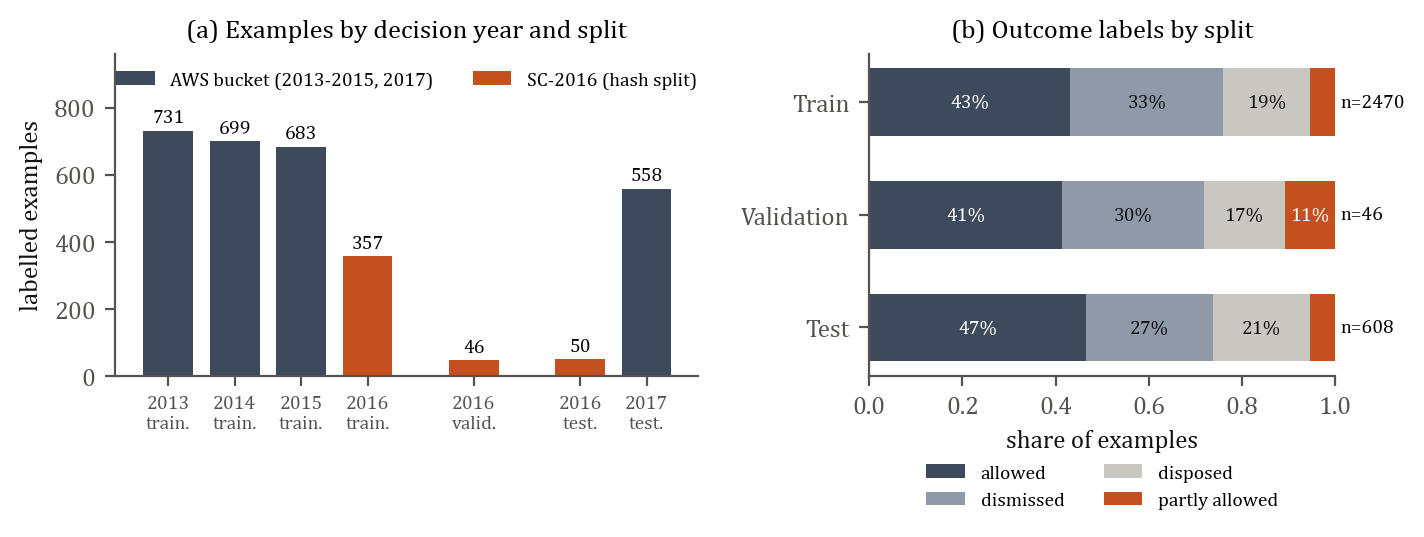
\includegraphics[width=.86\linewidth]{composition}
\caption{Benchmark composition. Panel (a) shows labelled examples by decision year, source and split, with the 2017 test year falling after all training years. Panel (b) shows the share of each outcome label per split.}\label{fig:composition}\end{figure}

\subsection{Selection audit}\label{sec:funnel}
Table~\ref{tab:audit} accounts for every archive judgment that was extracted, and it includes years beyond the original benchmark so that the benchmark years can be seen in context. Of 12,134 judgments, 10,334 are retained, which is a retention rate of 85.2\%. Within the benchmark itself, 426 of 3,142 archive judgments are lost to duplicate, year and label steps, and a further 45 are lost for lack of a usable view. Retention varies by year in ways that matter. The year 2009 lost 206 judgments for lack of a body marker, which appears to be a layout effect, while the test year 2017 retained 76.2\% against 85.6--89.6\% for the 2013--2015 training years. In particular, 89 of the 732 judgments from 2017 lacked a text phrase, against 24 to 63 per training year, so the test population may differ somewhat from the training population. Selection also changes class balance. Among rejected judgments from 2005--2015 that do have a four-way label, \cls{disposed} accounts for 46\% (266 of 576), compared with 16\% of retained judgments, and the benchmark therefore under-represents this class relative to the docket. The effect of the exclusions on task difficulty is measured in Section~\ref{sec:res-exclusions}.

\begin{table}[t]\centering\small
\caption{Selection audit for archive years by step. ``Other disposal'' has no four-way label. Two judgments counted under other disposal for 2013--2017 also appear in SC-2016, which accounts for the difference from the earlier figure of 162.}\label{tab:audit}
\setlength{\tabcolsep}{5pt}
\begin{tabular}{@{}lrrrrrrrr@{}}\toprule
Year(s) & Extracted & Duplicate & Other disposal & No phrase & Disagree & No view & Retained & \%\\\midrule
2005--2012 & 8,200 & 20 & 336 & 300 & 152 & 374 & 7,018 & 85.6\\
2013 & 854 & 3 & 35 & 63 & 15 & 7 & 731 & 85.6\\
2014 & 791 & 0 & 29 & 35 & 12 & 16 & 699 & 88.4\\
2015 & 762 & 1 & 31 & 24 & 11 & 12 & 683 & 89.6\\
2017 & 732 & 0 & 69 & 89 & 6 & 10 & 558 & 76.2\\
2018 & 795 & 0 & 127 & 17 & 6 & 0 & 645 & 81.1\\\midrule
All & 12,134 & 24 & 627 & 528 & 202 & 419 & 10,334 & 85.2\\\bottomrule
\end{tabular}\end{table}

\subsection{The masked input view}
Because judgments announce their own outcome, the input must exclude the passages that state it. An earlier version of our view began at the top of the document and exposed the headnote of the Supreme Court Reports, which summarises the holding in phrases such as ``Dismissing the appeal, the Court held'' and therefore leaks the answer directly. The final view, \texttt{body-prefix-masked-v2}, starts at the judgment body, which is located by the line recording delivery of the judgment, the jurisdiction block or an order heading. It takes at most 6,000 characters and never reads beyond 70\% of the document, so that a gap of at least 10\% always separates the view from the region used to derive the label. Every explicit disposition phrasing is replaced by the token \texttt{outcome\_phrase}, and judgments without a body marker or with fewer than 500 characters are excluded instead of being shown a view that might contain the headnote. The view therefore carries the facts, the procedural history and the beginning of the arguments, although it cannot remove implicit leakage, since a court's account of the facts may reflect its conclusion in ways that no phrase mask can detect.

\section{Method}\label{sec:method}
Figure~\ref{fig:arch} gives an overview of the system. Stage A builds a statute graph offline from eligible training judgments. Stage B prepares the masked input for each case and resolves its seed provisions. Stage C selects and encodes a subgraph into soft tokens, and Stage D passes those tokens and the prompt embeddings to the language model, which scores the four labels.

\begin{figure}[t]\centering\resizebox{\linewidth}{!}{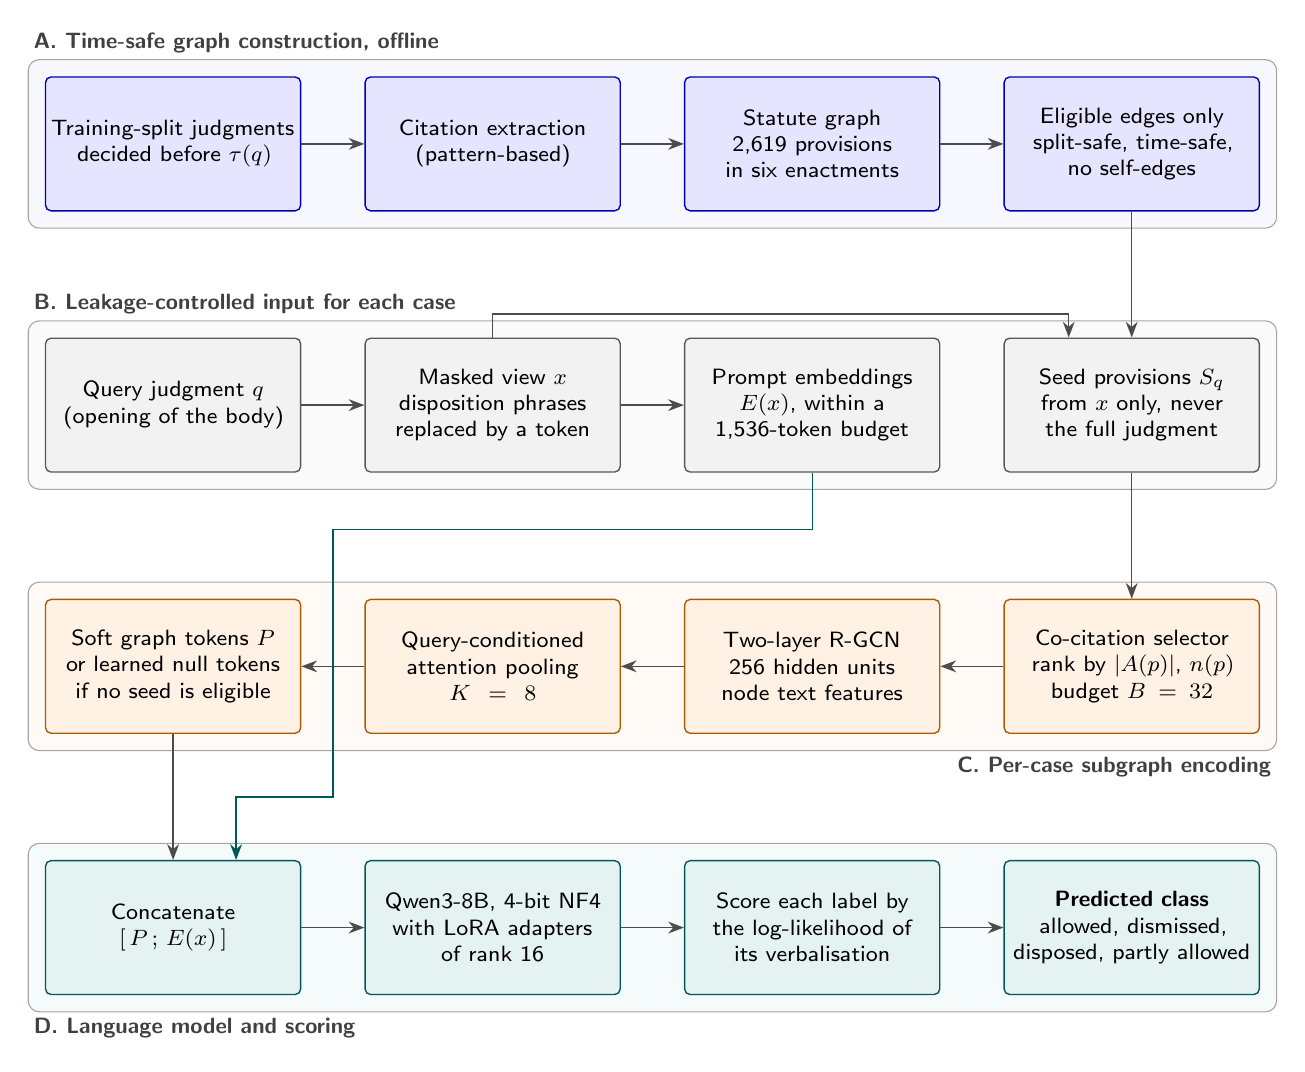
\begin{tikzpicture}[
  font=\sffamily\footnotesize, >={Stealth[length=2mm]}, line width=0.5pt,
  box/.style={draw=#1!70!black, fill=#1!10, rounded corners=2pt, align=center, minimum height=17mm, text width=31mm, inner sep=2pt},
  box/.default=gray,
  flow/.style={->, draw=black!70},
  lane/.style={draw=black!35, rounded corners=4pt, inner sep=6pt},
  lanelabel/.style={font=\sffamily\footnotesize\bfseries, text=black!75, anchor=south west, inner sep=2pt},
  note/.style={font=\sffamily\scriptsize, text=black!65, align=left}
]
% Row A: time-safe graph construction, left to right
\node[box=blue] (corpus) {Training-split judgments\\decided before $\tau(q)$};
\node[box=blue, right=8mm of corpus] (extract) {Citation extraction\\(pattern-based)};
\node[box=blue, right=8mm of extract] (kg) {Statute graph\\2,619 provisions\\in six enactments};
\node[box=blue, right=8mm of kg] (edges) {Eligible edges only\\split-safe, time-safe,\\no self-edges};
% Row D: leakage-controlled input, left to right
\node[box=gray, below=16mm of corpus] (raw) {Query judgment $q$\\(opening of the body)};
\node[box=gray, right=8mm of raw] (mask) {Masked view $x$\\disposition phrases\\replaced by a token};
\node[box=gray, right=8mm of mask] (prompt) {Prompt embeddings\\$E(x)$, within a\\1,536-token budget};
\node[box=gray, right=8mm of prompt] (seeds) {Seed provisions $S_q$\\from $x$ only, never\\the full judgment};
% Row B: subgraph encoding, right to left
\node[box=orange, below=16mm of seeds] (selector) {Co-citation selector\\rank by $|A(p)|$, $n(p)$\\budget $B=32$};
\node[box=orange, left=8mm of selector] (rgcn) {Two-layer R-GCN\\256 hidden units\\node text features};
\node[box=orange, left=8mm of rgcn] (pool) {Query-conditioned\\attention pooling\\$K=8$};
\node[box=orange, left=8mm of pool] (tokens) {Soft graph tokens $P$\\or learned null tokens\\if no seed is eligible};
% Row C: language model, left to right
\node[box=teal, below=16mm of tokens] (concat) {Concatenate\\$[\,P\,;\,E(x)\,]$};
\node[box=teal, right=8mm of concat] (llm) {Qwen3-8B, 4-bit NF4\\with LoRA adapters\\of rank 16};
\node[box=teal, right=8mm of llm] (score) {Score each label by\\the log-likelihood of\\its verbalisation};
\node[box=teal, right=8mm of score] (out) {\textbf{Predicted class}\\allowed, dismissed,\\disposed, partly allowed};
% flows inside lanes
\draw[flow] (corpus) -- (extract);
\draw[flow] (extract) -- (kg);
\draw[flow] (kg) -- (edges);
\draw[flow] (raw) -- (mask);
\draw[flow] (mask) -- (prompt);
\draw[flow] (selector) -- (rgcn);
\draw[flow] (rgcn) -- (pool);
\draw[flow] (pool) -- (tokens);
\draw[flow] (concat) -- (llm);
\draw[flow] (llm) -- (score);
\draw[flow] (score) -- (out);
% flows between lanes
\draw[flow] (edges) -- (seeds);
\draw[flow] (seeds) -- (selector);
\draw[flow] (tokens) -- (concat);
\draw[flow] (mask.north) -- ++(0,3mm) -| ([xshift=-8mm]seeds.north);
\coordinate (gap) at ($(tokens.east)!0.5!(pool.west)$);
\coordinate (mid1) at ($(prompt.south)!0.45!(rgcn.north)$);
\coordinate (mid2) at ($(tokens.south)!0.5!(concat.north)$);
\draw[flow, draw=teal!70!black] (prompt.south) -- (prompt.south |- mid1) -- (gap |- mid1) -- (gap |- mid2) -- ([xshift=8mm]concat.north |- mid2) -- ([xshift=8mm]concat.north);
% lanes
\begin{scope}[on background layer]
\node[lane, fill=blue!3, fit=(corpus)(edges)] (l1) {};
\node[lane, fill=black!2, fit=(raw)(seeds)] (l4) {};
\node[lane, fill=orange!4, fit=(selector)(tokens)] (l2) {};
\node[lane, fill=teal!4, fit=(concat)(out)] (l3) {};
\end{scope}
\node[lanelabel] at (l1.north west) {A. Time-safe graph construction, offline};
\node[lanelabel] at (l4.north west) {B. Leakage-controlled input for each case};
\node[lanelabel, anchor=north east] at (l2.south east) {C. Per-case subgraph encoding};
\node[lanelabel, anchor=north west] at (l3.south west) {D. Language model and scoring};
\end{tikzpicture}
}
\caption{Architecture of the statute co-citation graph prefix. The graph is built offline from eligible training judgments only, seeds come from the masked view and never from the full judgment, and the subgraph is encoded into eight soft tokens, or learned null tokens when no seed is eligible. The tokens are concatenated with the prompt embeddings before a 4-bit Qwen3-8B model with LoRA adapters scores each outcome label.}\label{fig:arch}\end{figure}

\subsection{Task and scoring}
Let $x$ be the masked view of a judgment and $\mathcal{Y}$ the set of four labels. The prompt consists of a fixed instruction, the view truncated to a 1,536-token budget and an answer cue, as shown in Appendix~\ref{app:prompt}. Given the prompt embedding sequence $E(x)$ and an optional graph prefix $P(x,G)$, the model scores each label by the total log-probability of its verbalisation $v_y$:
\begin{equation}
s(y\mid x)=\sum_{t=1}^{T_y}\log p_\theta\bigl(v_{y,t}\mid [P(x,G);E(x)],v_{y,<t}\bigr),\qquad \hat y=\arg\max_{y\in\mathcal{Y}}s(y\mid x).
\end{equation}
Scoring requires one forward pass over the prompt and short continuations for labels of more than one token, so the model always returns one of the four classes and cannot generate free text.

\subsection{Legal knowledge graph}
The graph $G=(V,E)$ is typed and backed by provenance, and its nodes are judgments, statute provisions, acts and the court. Citation edges run from a judgment to each provision it cites, containment edges run from an act to its provisions, and decision edges run from a judgment to the court. Citations are extracted by a pattern-based extractor that recognises references such as ``section 302 of the IPC'', ``Article 21'' and ``s.~482 CrPC'' and resolves each to a provision node. Every edge records the split of the judgment from which it was extracted and its date. In total the graph has 5,931 nodes and 17,076 edges, and training-split judgments contribute 9,173 citation edges that link 1,705 judgments to 996 distinct provisions. Most of these citations are to the IPC (3,722) and the Constitution (3,406), followed by the CrPC (1,593) and the IEA (452).

\subsection{Time-safe and split-safe retrieval}
For a query judgment $q$ with as-of date $\tau(q)$, an edge is eligible only if it was extracted from a training-split judgment, its date and the dates of its endpoints do not exceed $\tau(q)$, and neither endpoint is $q$ itself. We use the first day of the decision year as $\tau(q)$, which is conservative and also necessary because some SC-2016 judgments lack a full decision date. The seed set $S_q$ contains the provisions resolved from the masked view, never from the full judgment, that are eligible at $\tau(q)$. As a consequence, validation and test judgments never contribute edges, and no judgment decided after the query can influence its subgraph.

\subsection{Statute co-citation selector}
Let $C_q$ be the eligible training judgments and $\mathrm{Cit}(c)$ the set of provisions cited by judgment $c$. A provision $p\notin S_q$ becomes a candidate when some eligible judgment cites it together with a seed. For each candidate we record the seeds it is co-cited with and the number of supporting judgments:
\begin{equation}
A(p)=\bigcup_{c\in C_q:\,p\in\mathrm{Cit}(c)}\bigl(\mathrm{Cit}(c)\cap S_q\bigr),\qquad
n(p)=\bigl|\{c\in C_q:p\in\mathrm{Cit}(c),\ \mathrm{Cit}(c)\cap S_q\neq\emptyset\}\bigr|.
\end{equation}
Candidates are ranked by $|A(p)|$, then by $n(p)$, and then by identifier, and the selected node set consists of the seeds followed by the top-ranked candidates up to a budget of $B=32$ nodes. Two selected provisions are linked in both directions when an eligible judgment cites both. The construction is the legal analogue of bibliographic co-citation \cite{r31}, on the reasoning that provisions courts repeatedly invoke together, such as a penal section, the procedural provision under which an appeal is brought and the evidentiary rule on which it turns, describe the legal frame of a dispute. Judgment nodes are collapsed away, so that no case title, party name or outcome can enter the prefix. Our earlier selector, based on the PCST formulation of G-Retriever \cite{r23,r55}, produced subgraphs whose nodes were mostly co-citing judgments, and those judgments could contribute little beyond their titles.

\subsection{Graph encoder and soft-token prefix}
Each node $v$ has a feature vector $x_v\in\mathbb{R}^{4096}$, computed as the mean of the frozen LLM input embeddings over the first 48 tokens of the node's text, which is the provision's label and the first 400 characters of its content. After an input projection to $h=256$ dimensions, two relational graph convolution layers \cite{r32} update each node:
\begin{equation}
h_v^{(l+1)}=\mathrm{ReLU}\Bigl(W_0^{(l)}h_v^{(l)}+\sum_{r\in\mathcal{R}}\sum_{u\in\mathcal{N}_r(v)}\frac{1}{c_{v,r}}W_r^{(l)}h_u^{(l)}\Bigr),
\end{equation}
where $\mathcal{N}_r(v)$ is the set of neighbours of $v$ under relation $r$, $c_{v,r}=|\mathcal{N}_r(v)|$, and $\mathcal{R}$ includes inverse relations. The node states $H$ are then pooled into $K=8$ tokens by attention with learned queries $Q_0$, which are shifted by a projection of the mean prompt embedding $\bar e$ so that the pooling is conditioned on the query:
\begin{equation}
Q=Q_0+\mathbf{1}(W_q\bar e)^\top,\qquad \alpha=\mathrm{softmax}\bigl(Q(W_kH^\top)^\top\bigr),\qquad P=\gamma\cdot\mathrm{LN}(\mathrm{MLP}(\alpha H)).
\end{equation}
A two-layer perceptron maps the pooled states to the LLM's embedding space, and the learned scale $\gamma$ is initialised to the root-mean-square of the input embeddings, so that the prefix begins at the scale of ordinary tokens. When a query has no eligible seed, its subgraph is empty and the model receives $K$ learned null tokens, which means that every case receives the same eight prefix positions. The encoder has 6,340,097 parameters.

\subsection{Conditioning and training objective}
The prefix is concatenated before the prompt embeddings as $[P;E(x)]$. The base model is Qwen3-8B \cite{r59}, loaded in 4-bit NormalFloat with double quantisation and float16 computation \cite{r14}. LoRA adapters of rank 16, with $\alpha=32$ and dropout of 0.05, are attached to all attention and MLP projections \cite{r13}, which gives 43,646,976 trainable adapter parameters. Training minimises a class-weighted cross-entropy over the verbalised label and an end-of-sequence token:
\begin{equation}
L(x,y)=-w_y\sum_{t=1}^{T_y+1}\log p_\theta\bigl(v_{y,t}\mid[P;E(x)],v_{y,<t}\bigr),\qquad w_y\propto\frac{N}{|\mathcal{Y}|N_y},
\end{equation}
where the weights are inverse class frequencies normalised to a mean of one \cite{r60}, giving 0.58 for \cls{allowed}, 0.76 for \cls{dismissed}, 1.34 for \cls{disposed} and 4.61 for \cls{partly allowed}. Adapters and encoder are trained jointly with AdamW at learning rates of $2\times10^{-4}$ and $5\times10^{-4}$, using 10\% linear warm-up followed by linear decay, gradient accumulation over eight examples and gradient clipping at 1.0.

\subsection{Baselines and controls}
All LLM baselines share the same base model, prompt, input view and scoring rule. The majority baseline always predicts \cls{allowed}. The zero-shot baseline scores the four labels with the untuned model. The BM25 evidence prompt retrieves the four statute provisions most relevant to the view \cite{r63} and prepends up to 384 tokens of their text inside the same token budget, without training. The QLoRA text model is identical to the graph model except that it has no graph encoder, and it uses the same data, seed, data order, recipe and budget. In addition, the trained graph model is scored a second time with its graph tokens replaced by the null tokens, which isolates the per-case contribution of the subgraph at inference time.

On the development year we also use transparent linear controls. The reference model $T$ is a TF-IDF representation of one and two word sequences with class-balanced logistic regression. Model $S$ is a binary bag of the provisions cited in the view, which serves as a non-graph statute baseline, and model $G$ adds the co-citation neighbours chosen by the selector above. Models $T{+}S$ and $T{+}G$ join these blocks to the text. Two controls then test whether the content of the graph matters, with five random draws each. In $T{+}R$, the seeds of each case are replaced by the same number of provisions drawn according to citation frequency and then expanded, and in $T{+}H$, real seeds are expanded over a graph whose provision identifiers have been permuted. These controls test the information contained in the graph using a transparent model, and they do not test the R-GCN prefix inside an LLM.

\section{Experimental Setup}\label{sec:setup}
\subsection{Compute and software}
All LLM runs used a single NVIDIA T4 GPU with 16 GB of memory in a hosted notebook service, with PyTorch, Hugging Face Transformers \cite{r64}, PEFT and bitsandbytes. The base model is pinned to a fixed repository revision, and each notebook embeds the exact project code and configuration and verifies the SHA-256 of every input before training. Training writes resumable checkpoints every 96 examples, and one epoch over 2,470 examples took 7.38 hours for the text model and 7.43 hours for the graph model, so the prefix costs less than one percent of training time. Table~\ref{tab:config} summarises the configuration shared by the two models, which differ only in the variant and selector.

\begin{table}[t]\centering\small
\caption{Training configuration shared by the text and graph models.}\label{tab:config}
\begin{tabular}{@{}lY{9.3cm}@{}}\toprule Setting & Value\\\midrule
Base model & Qwen3-8B, 4-bit NF4, double quantisation, float16 computation\\
LoRA & rank 16, $\alpha=32$, dropout 0.05, on all attention and MLP projections\\
Learning rate & $2\times10^{-4}$ for LoRA and $5\times10^{-4}$ for the encoder, with AdamW\\
Schedule & 10\% warm-up, linear decay, one epoch, gradient accumulation of 8\\
Loss & inverse-frequency class weights, gradient clipping at 1.0\\
Input & masked body prefix of up to 6,000 characters, 1,536-token budget\\
Graph prefix & co-citation selector, 32-node budget, two R-GCN layers of 256 units, 8 tokens\\
Seed and order & 20261006, identical for both models\\\bottomrule
\end{tabular}\end{table}

\subsection{Evaluation protocol}
Each model is trained in its own session, which never reads test labels and records this fact in the run manifest. At the end of training the run is frozen, and a manifest records the SHA-256 of the adapter files, the encoder weights and the configuration. A separate evaluation session then takes the frozen run as input, verifies every hash, scores the test split exactly once and refuses to run again if a result already exists. Graph models are scored once more with their tokens ablated, and predictions for both test sources are produced in this single pass and reported separately. The later linear probes follow a written protocol in which each probe and its decision rule were fixed before any result was seen.

\subsection{Role of the validation set}
The validation set of 46 judgments was used to monitor training and to choose among development designs, including the move from PCST to the statute selector and the choice of training recipe, and it was never used for decisions at test time. This is a real weakness of the study, because a set of this size offers very little evidence for model selection or hyperparameter decisions. Early stopping, the choice of epoch and the choice among designs of similar quality should therefore be read as close to arbitrary, and the extent of the problem is quantified in Section~\ref{sec:res-valsize}. For this reason the later linear probes use a much larger development year in place of the validation set.

\subsection{Metrics and statistics}
Macro-averaged F1 over the four classes is the primary metric because the classes are imbalanced, and we also report accuracy together with per-class precision, recall and F1. Confidence intervals are 95\% percentile bootstrap intervals over cases with 10,000 resamples \cite{r34}. Paired comparisons resample cases jointly for both systems and report the interval of the difference \cite{r28}, and accuracy differences are also tested with the exact McNemar test on discordant cases \cite{r35}. Development probes use 2,000 resamples and a pre-registered rule under which a change is adopted only when it gains at least 0.03 in macro-F1 and its interval excludes zero.

\section{Result Analysis}\label{sec:results}
\subsection{Main results on the test sets}
Table~\ref{tab:main} and Figure~\ref{fig:scores} report every LLM system on the two test sources and on their union. Because \cls{allowed} is the most frequent class, the majority baseline reaches an accuracy of 0.465 but a macro-F1 of only 0.159. Both fine-tuned models more than double that macro-F1 on 2017 and on the full test set, reaching 0.360 for text and 0.365 for the graph model across all 608 cases. Fine-tuning is clearly beneficial relative to the untrained model, which scores 0.269 and rarely predicts \cls{disposed} (30 of 608 predictions). Prepending BM25-retrieved statute text raises accuracy to 0.438 only by pushing predictions towards \cls{allowed} (425 of 608), and macro-F1 falls to 0.255. Table~\ref{tab:paired} shows that both fine-tuned models improve on both untrained baselines by about 0.09 to 0.11 in macro-F1, with intervals that exclude zero.

\begin{table}[t]\centering\small
\setlength{\tabcolsep}{4pt}
\caption{Test results from a single evaluation of frozen models on the SC-2016 ($n=50$), 2017 ($n=558$) and combined ($n=608$) sets. Brackets give 95\% bootstrap intervals for macro-F1 (mF1). Each LLM row is a single training run.}\label{tab:main}
\begin{tabular}{@{}lcccccc@{}}\toprule
System & \multicolumn{2}{c}{SC-2016} & \multicolumn{2}{c}{2017} & \multicolumn{2}{c}{All}\\
& Acc & mF1 & Acc & mF1 [95\% CI] & Acc & mF1 [95\% CI]\\\midrule
Majority & .500 & .167 & .462 & .158 & .465 & .159\\
Zero-shot & .340 & .250 & .367 & .268 [.232, .305] & .365 & .269 [.233, .303]\\
BM25 prompt & .320 & .211 & .448 & .259 [.229, .289] & .438 & .255 [.227, .284]\\
QLoRA text & .440 & .316 & .489 & .365 [.322, .409] & .485 & .360 [.320, .400]\\
QLoRA + graph & .320 & .226 & .462 & .379 [.330, .430] & .451 & .365 [.320, .412]\\
Graph tokens removed & .320 & .223 & .461 & .378 [.329, .427] & .449 & .364 [.319, .407]\\\bottomrule
\end{tabular}\end{table}

\begin{figure}[t]\centering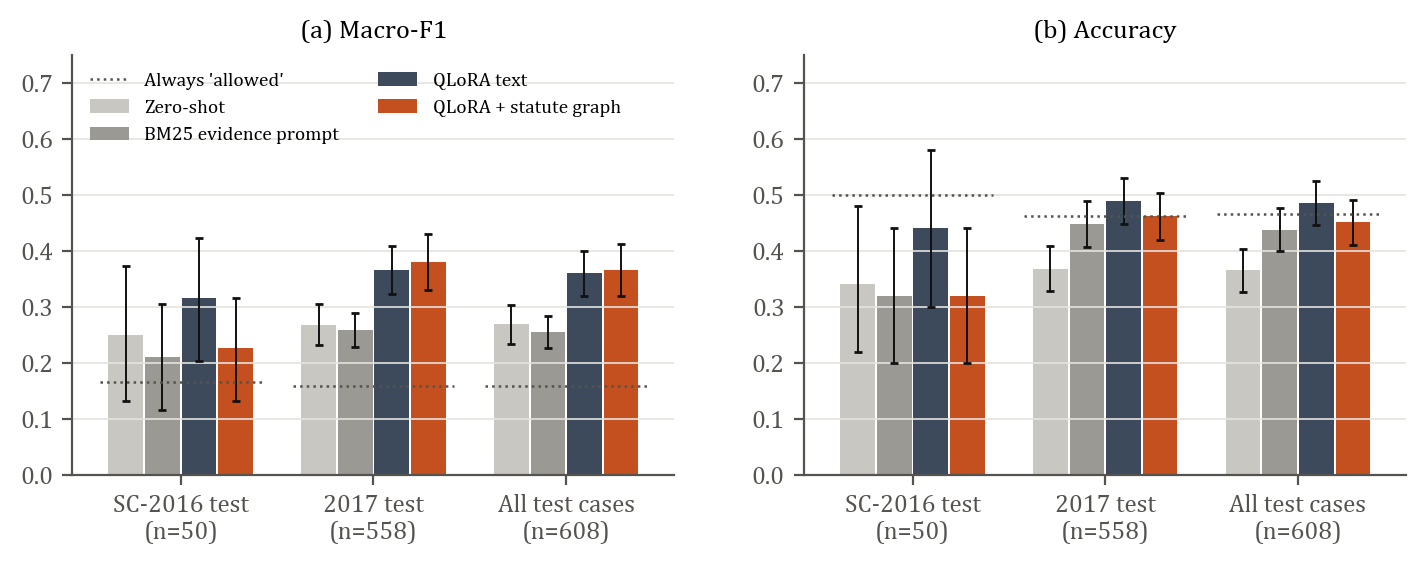
\includegraphics[width=.95\linewidth]{test-scores}
\caption{Test macro-F1 (a) and accuracy (b) for each system and test source with 95\% bootstrap intervals. The dotted line marks the majority baseline.}\label{fig:scores}\end{figure}

\begin{table}[t]\centering\small
\setlength{\tabcolsep}{4pt}
\caption{Paired differences (first system minus second) on the same test cases, with 95\% paired bootstrap intervals. The value $p$ is from the exact McNemar test on accuracy.}\label{tab:paired}
\begin{tabular}{@{}llccc@{}}\toprule
Comparison & Test set & $\Delta$ macro-F1 [95\% CI] & $\Delta$ accuracy [95\% CI] & $p$\\\midrule
Graph $-$ text & 2017 ($n=558$) & +.014 [$-$.028, +.058] & $-$.027 [$-$.065, +.011] & .20\\
& SC-2016 ($n=50$) & $-$.090 [$-$.179, $-$.007] & $-$.120 [$-$.220, $-$.020] & .07\\
& All ($n=608$) & +.006 [$-$.034, +.046] & $-$.035 [$-$.071, +.002] & .08\\
Text $-$ zero-shot & All & +.090 [+.037, +.143] & +.120 [+.069, +.171] & $<$.001\\
Graph $-$ zero-shot & All & +.096 [+.038, +.153] & +.086 [+.031, +.140] & .003\\
Graph $-$ BM25 prompt & All & +.110 [+.056, +.164] & +.013 [$-$.043, +.067] & .677\\
Graph $-$ tokens removed & All & +.002 [$-$.022, +.021] & +.002 [$-$.013, +.016] & 1.00\\\bottomrule
\end{tabular}\end{table}

The comparison between the graph and text models is the central result. On 2017 the graph model's macro-F1 point estimate is higher by 0.014, but the interval runs from $-$0.028 to +0.058, comfortably including zero and effects of either sign, and accuracy points the other way at $-$0.027. On the smaller SC-2016 set the text model leads, with a macro-F1 interval that excludes zero and $p=0.07$ on accuracy, and pooled over all 608 cases the two models are level. An earlier version of this manuscript described the graph model as the best system on 2017. That ranking is not supported, because it rests on a single-run point estimate inside its own interval, and the comparison set did not contain a strong non-LLM baseline on the same cases.

\subsection{Per-class behaviour}
Table~\ref{tab:perclass} gives precision, recall and F1 for each class, and Table~\ref{tab:confusion} gives the confusion matrices. Per-class values for the QLoRA models on the 2017 and SC-2016 sets were reconstructed from the reported gold and predicted counts, class F1 values and combined matrices, and every reconstructed row reproduces its reported accuracy and macro-F1. The separate off-diagonal counts for those two sets, and per-class values for the zero-shot, BM25 and ablated systems, require per-case outputs that are not in our current repository. We therefore report only accuracy and macro-F1 for those systems, as in Table~\ref{tab:main}, and we have not estimated the missing values from charts.

\begin{table}[t]\centering\footnotesize
\setlength{\tabcolsep}{3.5pt}
\caption{Per-class precision/recall/F1. $^\dagger$Different test year and training data (2005--2015 and 2017), so this is not a paired comparison. The majority baseline on all 608 cases scores .47/1.00/.63 on allowed and zero on other classes, with accuracy .465 and macro-F1 .159.}\label{tab:perclass}
\begin{tabular}{@{}llccccrr@{}}\toprule
System & Test set & allowed & dismissed & disposed & partly allowed & Acc & mF1\\\midrule
QLoRA text & 2017 (558) & .57/.70/.63 & .42/.20/.27 & .41/.49/.45 & .11/.11/.11 & 0.489 & 0.365 \\
QLoRA + graph & 2017 (558) & .58/.52/.55 & .49/.33/.40 & .33/.58/.42 & .25/.11/.15 & 0.462 & 0.379 \\
QLoRA text & SC-2016 (50) & .64/.56/.60 & .50/.18/.27 & .29/.67/.40 & .00/.00/.00 & 0.440 & 0.316 \\
QLoRA + graph & SC-2016 (50) & .53/.36/.43 & .14/.09/.11 & .25/.67/.36 & .00/.00/.00 & 0.320 & 0.226 \\
QLoRA text & All (608) & .58/.69/.63 & .42/.20/.27 & .40/.50/.44 & .10/.09/.10 & 0.485 & 0.360 \\
QLoRA + graph & All (608) & .58/.51/.54 & .47/.32/.38 & .32/.59/.42 & .21/.09/.13 & 0.451 & 0.365 \\
TF-IDF + LR$^\dagger$ & 2018 (645) & .52/.48/.50 & .45/.35/.39 & .46/.59/.51 & .21/.40/.28 & 0.460 & 0.421 \\
\bottomrule\end{tabular}\end{table}

\begin{table}[t]\centering\footnotesize
\caption{Confusion matrices, with rows as actual classes and columns as predicted classes (A allowed, D dismissed, Dp disposed, P partly allowed).}\label{tab:confusion}
\setlength{\tabcolsep}{3pt}
\begin{tabular}{@{}l*{4}{>{\raggedleft\arraybackslash}p{0.72cm}}@{\hskip 8pt}*{4}{>{\raggedleft\arraybackslash}p{0.72cm}}@{\hskip 8pt}*{4}{>{\raggedleft\arraybackslash}p{0.72cm}}@{}}\toprule
& \multicolumn{4}{c}{QLoRA text (All, 608)} & \multicolumn{4}{c}{QLoRA + graph (All, 608)} & \multicolumn{4}{c}{TF-IDF + LR (2018, 645)}\\
& A & D & Dp & P & A & D & Dp & P & A & D & Dp & P\\\midrule
A & 195 & 30 & 47 & 11 & 144 & 42 & 93 & 4 & 130 & 57 & 59 & 25\\
D & 75 & 33 & 42 & 15 & 51 & 52 & 55 & 7 & 73 & 67 & 42 & 12\\
Dp & 51 & 11 & 64 & 1 & 42 & 10 & 75 & 0 & 34 & 20 & 88 & 8\\
P & 18 & 4 & 8 & 3 & 12 & 7 & 11 & 3 & 11 & 4 & 3 & 12\\\bottomrule
\end{tabular}\end{table}

The graph run moves predictions on 2017 away from \cls{allowed} (232 against 317, with 258 gold cases) and towards \cls{disposed} (210 against 140, with 118 gold cases) and \cls{dismissed} (104 against 74, with 154 gold cases). This shift lifts dismissed recall from 0.20 to 0.33 and dismissed F1 from 0.272 to 0.395, while allowed F1 falls from 0.630 to 0.551, disposed F1 falls from 0.450 to 0.421, and the over-prediction of \cls{disposed} worsens. No test was specified in advance for per-class differences, and a shift in class balance between two single runs is exactly what an arbitrary perturbation of training could produce. We therefore report the shift as an observation and attach no causal claim to it. Figure~\ref{fig:classes} shows the same pattern across all 608 test cases.

\begin{figure}[t]\centering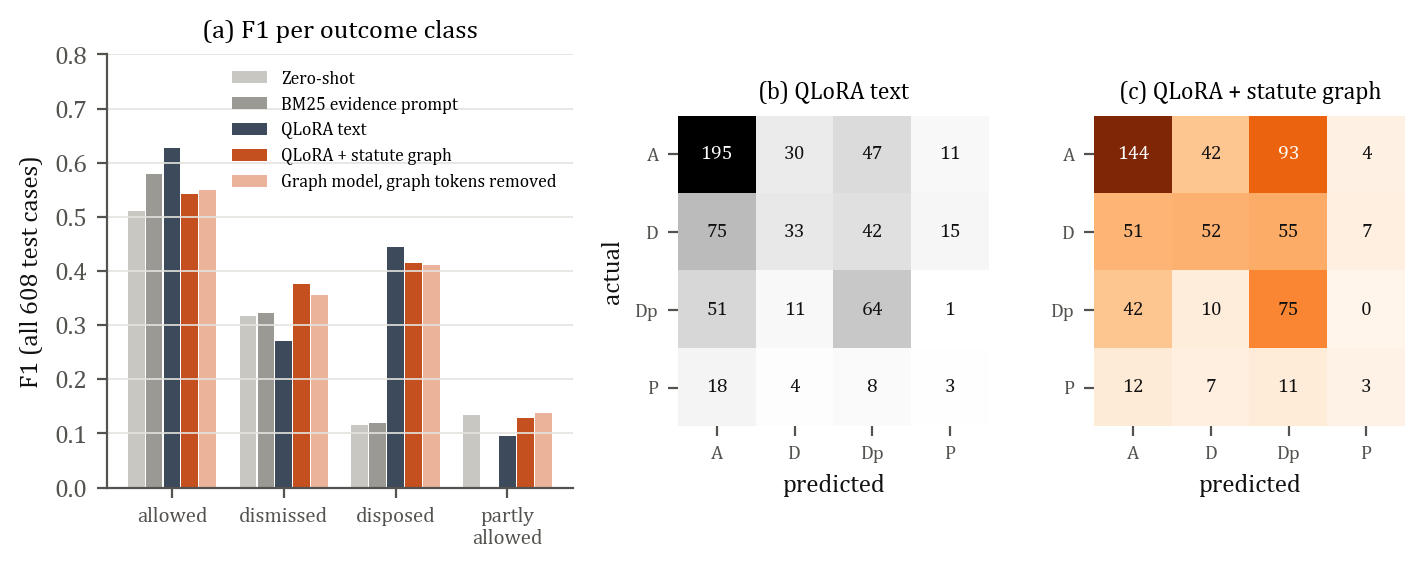
\includegraphics[width=.9\linewidth]{classes}
\caption{Panel (a) shows F1 per class on all 608 test cases, and panels (b) and (c) show the confusion matrices of the text and graph models.}\label{fig:classes}\end{figure}

\subsection{Graph coverage, subgroups and ablation}
A graph prefix can be informative only when the view cites an eligible provision. Coverage is 44.8\% of training cases, 39.1\% of validation cases and 35.9\% of test cases (218 of 608), and a non-empty subgraph grows from about 3.0 seeds to 31.7 provisions on average, with 855 directed co-citation edges (Figure~\ref{fig:coverage}).

\begin{figure}[t]\centering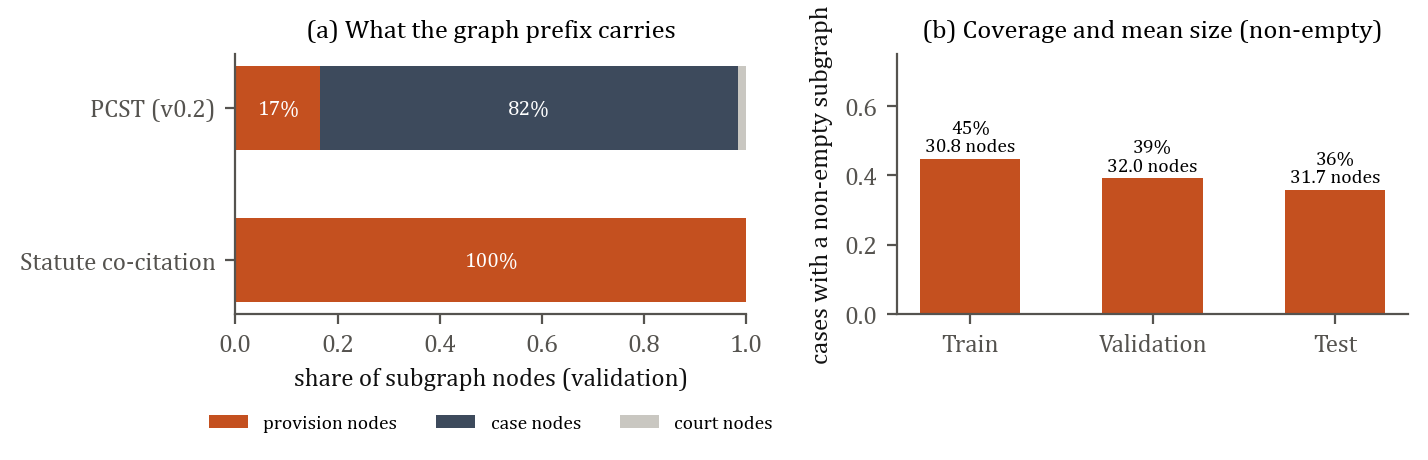
\includegraphics[width=.8\linewidth]{coverage}
\caption{Panel (a) shows the node composition of validation subgraphs under the earlier PCST selector and the statute selector, and panel (b) shows the share of cases with a non-empty subgraph and the mean subgraph size per split.}\label{fig:coverage}\end{figure}

\begin{table}[t]\centering\small
\caption{Test results by subgraph availability (accuracy / macro-F1). Without a subgraph the graph and ablated models coincide by construction.}\label{tab:subgroup}
\begin{tabular}{@{}lrccc@{}}\toprule
Subset & $n$ & QLoRA text & QLoRA + graph & Tokens removed\\\midrule
With subgraph & 218 & .472 / .381 & .450 / .403 & .445 / .385\\
Without subgraph & 390 & .492 / .334 & .451 / .334 & .451 / .334\\\bottomrule
\end{tabular}\end{table}

On the 218 cases with a subgraph (Table~\ref{tab:subgroup}), the graph minus text difference is +0.022 with an interval of $-$0.048 to +0.093, which cannot be distinguished from zero. On the 390 cases without a subgraph, the graph model loses 0.041 in accuracy to the text model despite receiving no per-case graph input at all, while macro-F1 ties at 0.334. That accuracy gap cannot come from graph content, so it is direct evidence that the two runs differ for reasons other than per-case graph information. Removing the graph tokens changes 32 predictions (5.3\%), all among cases with a subgraph, and changes macro-F1 by +0.002 with an interval of $-$0.022 to +0.021. Comparing cases with and without a subgraph against each other would be misleading, because the two groups differ in composition. In the linear data reported next, text alone scores 0.482 on cases with a subgraph and 0.338 on cases without one, although no graph is involved.

\subsection{Linear controls on the development year}\label{sec:controls}
Table~\ref{tab:controls} reports the pre-registered controls on the 683 development cases from 2015, and no later year was scored. No candidate passes the adoption rule. Cited statutes carry real signal on their own, reaching 0.301 against a floor of 0.149, yet they contribute nothing when added to text, and co-citation neighbours add nothing further, with $T{+}G$ minus $T{+}S$ at 0.000 (interval $-$0.005 to +0.006) on the wider training window. Real graphs also do no better than randomised statutes or shuffled edges, since $T{+}G$ minus the first draw of $T{+}R$ is +0.003 (interval $-$0.006 to +0.011) and minus the first draw of $T{+}H$ is $-$0.002 (interval $-$0.009 to +0.005). The block weights were both chosen at the lowest grid value on an inner split where every block scored below text, so these differences are small partly by construction. The conclusion that the blocks do not help nevertheless stands, because no weight on the grid improved on text alone.

\begin{table}[t]\centering\small
\setlength{\tabcolsep}{4pt}
\caption{Linear statute and graph controls on development year 2015 ($n=683$). Delta is macro-F1 against $T$ with a 95\% paired interval. Rows $R$ and $H$ give the mean and standard deviation over five draws.}\label{tab:controls}
\begin{tabular}{@{}lcccc@{}}\toprule
& \multicolumn{2}{c}{Train 2005--2014 (8,448)} & \multicolumn{2}{c}{Train 2013--2014 (1,430)}\\
Features & mF1 & Delta & mF1 & Delta\\\midrule
$T$: TF-IDF text & .409 & & .395 & \\
$S$: cited provisions only & .301 & & .272 & \\
$G$: provisions and co-citation neighbours & .271 & & .230 & \\
$T{+}S$: non-graph statute baseline & .403 & $-$.006 [$-$.014, .000] & .395 & .000 [$-$.003, +.004]\\
$T{+}G$: text and graph & .403 & $-$.006 [$-$.013, .000] & .390 & $-$.005 [$-$.012, +.001]\\
$T{+}R$: randomised statutes & .405 (.003) & & .391 (.002) & \\
$T{+}H$: shuffled edges & .406 (.002) & & .395 (.001) & \\\bottomrule
\end{tabular}\end{table}

The subgroup results point the same way. With training on 2005--2014, $T{+}G$ minus $T$ is $-$0.005 (interval $-$0.020 to +0.005) on the 261 cases with a subgraph and $-$0.007 (interval $-$0.015 to 0.000) on the 422 cases without one, so there is no sign of a benefit concentrated where the graph exists. Because a linear fit has no random seed of its own, we also redrew the 2013--2014 training cases ten times to measure sensitivity to the training sample. The gap between $T{+}G$ and $T$ then has a mean of +0.001 and a standard deviation of 0.005, and it is positive in five of the ten resamples, while each model's own macro-F1 varies from about 0.30 to 0.36. This measures sensitivity to the data only, and it is no substitute for measuring seed variance in the LLMs.

\subsection{Other neural baselines and the linear reference}
Table~\ref{tab:baselines} summarises the development-year baselines. No frozen embedding model and no fine-tuned InLegalBERT model beats TF-IDF, and averaging their probabilities with TF-IDF adds nothing detectable. A TF-IDF model fixed in advance and trained on 2005--2015 and 2017 was then scored once on 645 cases decided in 2018, reaching a macro-F1 of 0.421 (interval 0.376 to 0.465) and an accuracy of 0.460 (interval 0.422 to 0.499). This is a different test year with more training data, so it is not a paired comparison with Table~\ref{tab:main}. It does mean, however, that we cannot claim the fine-tuned LLMs exceed a linear baseline.

\begin{table}[t]\centering\small
\caption{Development-year baselines on 2015 ($n=683$). Deltas are against TF-IDF on the same training window, with 95\% paired intervals.}\label{tab:baselines}
\begin{tabular}{@{}llcc@{}}\toprule
Model & Train & mF1 & Delta\\\midrule
TF-IDF + LR & 2013--14 and 2005--14 & .395 and .415 & \\
InLegalBERT frozen + LR & 2005--14 & .314 & $-$.101 [$-$.146, $-$.051]\\
Qwen3-Embedding-0.6B frozen + LR & 2005--14 & .274 & $-$.140 [$-$.193, $-$.084]\\
InLegalBERT fine-tuned (two seeds) & 2005--14 & .350 and .387 & $-$.065 and $-$.028\\
SaulLM-7B frozen + LR & 2013--14 & .345 & $-$.050 [$-$.106, +.006]\\
SaulLM-7B frozen + LR & 2008--14 & .352 & $-$.064 [$-$.113, $-$.013]\\\bottomrule
\end{tabular}\end{table}

\subsection{Input, data, framing and labels}
Macro-F1 of the TF-IDF model changes little with the input view, moving by $-$0.007 (interval $-$0.037 to +0.025) with a 24,000-character view and by $-$0.013 (interval $-$0.042 to +0.018) with the whole body up to the 70\% cap. Widening training from 2013--14 to 2005--14 gives +0.012 (interval $-$0.043 to +0.068). Random training subsets rise until about 4,500 cases and then flatten near 0.41, and part of the earlier slope reflected recency, since 1,430 random cases from 2005--14 score 0.343 against 0.395 for the 1,430 cases of 2013--14. Header metadata and recency weighting also failed the adoption rule, with a best result of +0.013 (interval $-$0.016 to +0.042).

The leakage audit supports the masked view. On the development year no view contains a literal disposition phrase after masking, although 65--91\% of views, depending on view type, contain outcome words such as \emph{allow} or \emph{dismiss} in other contexts. A model using only those words reaches a macro-F1 of 0.232, and removing them from the baseline leaves it effectively unchanged at 0.396 against 0.395. The signal therefore does not come from residual outcome words, and the top TF-IDF features are topical, such as \emph{insurance company}, \emph{arms act} and \emph{compensation}.

Task framing moves results the most, as Table~\ref{tab:framing} shows, although scores across framings are not directly comparable because each framing has its own floor. For label quality, a reader examined a random sample of 40 \cls{disposed} and 25 \cls{partly allowed} endings from training years. The reader was an LLM assistant and not a lawyer, so the following estimates are rough and need expert review. About half of the \cls{disposed} sample formed a coherent class of directions with no clear winner, whereas about 40\% would fit another label equally well, such as partial relief, remand or mixed batches. All 25 \cls{partly allowed} endings were partial relief, but similar outcomes also appear under \cls{disposed}. A rule-based relabelling agreed with a blind reading on only 26 of 40 fresh cases and was dropped before any model used it.

\begin{table}[t]\centering\small
\setlength{\tabcolsep}{4pt}
\caption{Task framings with TF-IDF and logistic regression. Development is 2015 with 2013--14 training, test is the single 2018 evaluation, and the floor is always-allowed macro-F1 on test.}\label{tab:framing}
\begin{tabular}{@{}lccccc@{}}\toprule
Framing & Dev Acc & Dev mF1 & Test Acc & Test mF1 [95\% CI] & Floor\\\midrule
Four-way & .499 & .395 & .460 & .421 [.376, .465] & .148\\
Three-way (partly merged into allowed) & .521 & .451 & .515 & .502 [.461, .540] & .212\\
Binary, allowed against dismissed & .624 & .593 & .620 & .602 [.556, .645] & .378\\\bottomrule
\end{tabular}\end{table}

\subsection{Effect of exclusions on difficulty}\label{sec:res-exclusions}
The exclusions probably make the benchmark somewhat easier, by a measurable but modest amount. On the 2015 development year, 33 cases have a four-way official label and a usable view but failed the text rule, and they score an accuracy of 0.303 and a macro-F1 of 0.233, against 0.455 and 0.409 for the retained cases. Including them lowers macro-F1 by 0.007, to 0.402 on 716 cases, although an estimate from 33 cases is rough. The largest unknown is the group of 627 other-disposal judgments, which have no four-way label, cannot be scored and therefore lie outside anything the benchmark can say.

\subsection{Time and text pipeline}\label{sec:res-time}
Temporal effects can be examined inside a single text pipeline, because all archive cases are PDF text. A model trained on 2005--2009 scores 0.376, 0.370, 0.395, 0.346, 0.368 and 0.399 on the years 2010 to 2015, which shows no clear trend. Rolling two-year training windows score 0.377, 0.363 and 0.359 at one, two and three years ahead, with a standard deviation across years of about 0.02. Temporal decay in a linear model is therefore about 0.02 over two years, which is small beside the difference of 0.104 between the graph minus text gaps on the two test sets.

\subsection{What 46 validation cases can resolve}\label{sec:res-valsize}
To quantify the weakness of the validation set, we drew 46 cases at random from the 683 development cases 5,000 times. A model with a macro-F1 of 0.409 on all 683 cases ranges from 0.232 to 0.584 across 95\% of draws, with a standard deviation of 0.093. Two models with a true gap of 0.014 swap order in 47\% of draws, and their observed difference ranges from $-$0.196 to +0.224. A difference smaller than about 0.2 on 46 cases is therefore uninformative, and this applies to most of the differences in the development history below.

\subsection{Development history and training dynamics}
Table~\ref{tab:dev} lists every 8B development run on the 46 validation cases. In light of the previous subsection, the table is a record of what was tried and offers no evidence that any change caused an improvement, and the final graph minus text validation gap is $-$0.020 with an interval of $-$0.111 to +0.075. The PCST subgraphs were dominated by co-citing judgments, which made up 251 of 307 nodes and were represented only by their titles, and this observation motivated the move to provision-only subgraphs as a matter of design rationale, not of measured benefit. Figure~\ref{fig:loss} shows training loss for the two final runs, which see the same examples in the same order. The final 100-example loss is 0.580 for the text model and 0.590 for the graph model, and neither run recorded a non-finite loss or gradient.

\begin{table}[t]\centering\small
\caption{Development history on the 46-case validation set. Data v0.2 has 357 SC-2016 training examples and v0.3 has 2,470. The original recipe is unweighted with a constant learning rate, and the balanced recipe adds class weights, a schedule and gradient clipping.}\label{tab:dev}
\begin{tabular}{@{}lllccc@{}}\toprule
Model & Data & Recipe & Epochs & Acc & mF1\\\midrule
Qwen3-8B zero-shot & n/a & none & 0 & .348 & .318\\
Qwen3-8B + BM25 & n/a & none & 0 & .391 & .214\\
Qwen3-8B text & v0.2 & original & 3 & .565 & .441\\
Qwen3-8B graph (PCST) & v0.2 & original & 3 & .435 & .244\\
Saul-7B text & v0.2 & original & 3 & .435 & .183\\
Qwen3-8B text & v0.2 & balanced & 3 & .478 & .377\\
Qwen3-8B graph (PCST) & v0.2 & balanced & 3 & .435 & .283\\
Qwen3-8B text & v0.3 & balanced & 1 & .457 & .405\\
Qwen3-8B graph (statute) & v0.3 & balanced & 1 & .413 & .385\\\bottomrule
\end{tabular}\end{table}

\begin{figure}[t]\centering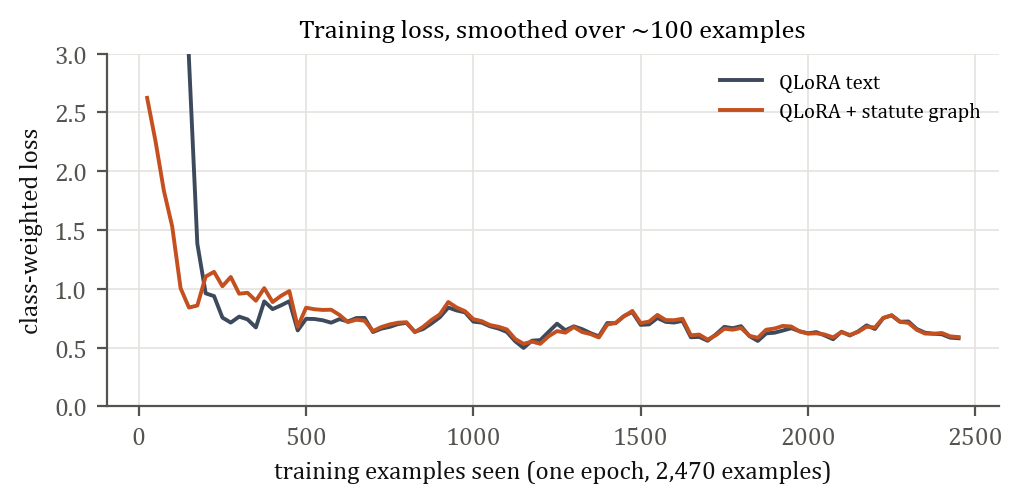
\includegraphics[width=.62\linewidth]{loss}
\caption{Class-weighted training loss, smoothed over about 100 examples, for the two final models.}\label{fig:loss}\end{figure}

\section{Discussion}\label{sec:discussion}
\subsection{What the fine-tuned models learn}
A QLoRA-adapted Qwen3-8B learns a usable signal from the masked opening, and its improvement over the untrained model is statistically secure. The evidence on the nature of that signal suggests that it reflects case type and procedural posture more than any assessment of the merits, because the strongest linear features are topical and a bag-of-words model reaches the same range. Classifying from a masked opening is much harder than reading the outcome from the operative order, yet for the reasons given in the Introduction it should not be confused with forecasting a decision.

\subsection{Where the limits lie}
Across models ranging from a bag of words to fine-tuned 8B LLMs, no system we tested moves far beyond the same modest range of four-way performance. More data and longer views help little beyond a few thousand cases, whereas framing and label definition move results much more. The limit therefore seems to lie in the input and the definition of the task more than in the capacity of the model.

The four-class formulation is a research choice and is not required by any practical use case that we can identify. It reflects the Registry's own disposal categories, retains procedural dispositions that binary benchmarks discard and supports direct audit against official metadata. Since the framing substantially changes performance and part of the \cls{disposed} class appears to overlap with others, we report three-way and binary framings beside it, and we suggest that any future practical study should define its classes together with practitioners. The four-way numbers are retained for comparability and not because the formulation is privileged.

\subsection{Separating pipeline effects from time}
The two test sets differ in several respects at once, and this limits what can be concluded from any comparison between them. The SC-2016 test cases come from 2016 through an OCR pipeline used by 14\% of the training data, whereas the 2017 cases come a year later through the PDF pipeline used by 86\% of the training data, and the sets also differ tenfold in size. The difference in graph minus text gaps between them may reflect the pipeline, the year, selection or sampling noise, and a single run cannot apportion it. We also withdraw the earlier inference that the closeness of test and validation scores shows little drift, because the validation set is far too small to support it. The single-pipeline analysis in Section~\ref{sec:res-time} puts a rough scale on the effect of time and suggests that time alone does not explain the SC-2016 gap, but it does not measure the pipeline effect directly, which would require scoring the same judgments under both pipelines with the frozen models.

\subsection{Limitations}\label{sec:limits}
Several limitations qualify these findings, and the first two bear directly on the central question. Each final LLM configuration was trained only once and for one epoch, so seed variance is unmeasured, the paired intervals capture sampling over test cases alone, and conclusions about the graph are provisional until matched seeds have been run. Randomised and shuffled controls exist only for linear models on the development year, and those models test the information in the graph without testing the prefix itself, so a linear model could miss interactions that a graph encoder might exploit. The LLMs and TF-IDF have not been compared on the same cases, because the linear test result comes from a different year.

The remaining limitations concern the data. The 46-case validation set underlies the development choices. Labels depend on a phrase rule and on official metadata, selection removes harder cases and under-represents \cls{disposed}, and the label audit was not carried out by a lawyer. Only a minority of test cases receive a subgraph, which reflects both citation extraction and the restriction to six enactments, so a broader graph remains untested. Per-class data are incomplete for the zero-shot, BM25 and ablated systems. Finally, we did not measure expert performance on these masked views, so \textbf{performance relative to human judgment remains unknown} and we cannot say how hard the task is for a trained lawyer.

\subsection{Ethical considerations}
All judgments are public records released for reuse, and the graph prefix excludes case titles and party names by construction. Outcome classifiers should not be used to decide cases or to advise litigants without professional oversight, particularly because errors are distributed unevenly across outcome classes and LLMs can produce confident but unfounded legal statements \cite{r51}. We present these models as research instruments for studying legal structure and evaluation methodology, and not as decision aids.

\section{Further Research}\label{sec:future}
The most important next step is to train the text, graph and randomised-prefix models across matched seeds and to evaluate them on the unopened 2019 data, because this is the necessary test of the second research question. A paired linear baseline on the same cases as the LLMs would settle whether the language models improve on a simple classifier, and an expert baseline on a sample of masked views would place all of these scores in context. Beyond these, the label problem deserves direct attention through case-by-case annotation of \cls{disposed} by legal experts, reported beside the four-way numbers and never in place of them.

Other directions depend on the outcome of those experiments. Inputs drawn from before the decision, such as filings and lower-court orders, would permit a real evaluation of pre-decision classification. Citation extraction could be improved and further enactments added to raise graph coverage, and time-safe precedent signals \cite{r50} could be tested, although these extensions are justified only if the basic controls show that the current graph has an effect. Scoring identical judgments under OCR and PDF text would measure the pipeline effect directly, and rhetorical-role segmentation \cite{r41} could help to select facts and arguments from anywhere before the decision under explicit leakage audits.

\section{Conclusion}\label{sec:conclusion}
We built a leakage-controlled, out-of-time benchmark for four-way outcome classification at the Supreme Court of India and used it to test a statute co-citation graph prefix for a quantised language model. Fine-tuning clearly helps relative to an untrained model, but the graph prefix shows no detectable added value, either in the paired LLM comparison or in linear controls where randomised statutes and shuffled edges perform as well as the real graph. A simple linear baseline reaches the same range as the language models, and the limits on performance seem to lie in the input and the definition of the task. These conclusions remain provisional in one important respect, because seed variance and a randomised control for the language model have yet to be measured.

\section*{Data and Code Availability}
Both judgment sources and the statute sources are public \cite{r29,r30,r62}. The project repository contains the code that downloads, extracts, cleans, labels and splits the data, builds the graph and runs the experiments, together with the source registry and configurations. Run manifests recorded the SHA-256 of the corpus (d92f9dd3\ldots), training manifest (7b5c2c2f\ldots), graph (c5a733cd\ldots) and base-model revision (b968826d\ldots). The development-year probes and the 2018 evaluation can be reproduced from the repository's notebooks, while per-case predictions of the frozen LLM runs are not part of the current repository.

\section*{Acknowledgements}
We thank the maintainers of the open judgment archive and of the SC-2016 collection for making the data available, and the providers of the hosted GPU notebooks used for all experiments.

\appendix
\section{Prompt and label verbalisers}\label{app:prompt}
\begin{quote}\small
Read the opening of an Indian Supreme Court judgment. Phrases that state the final disposition have been replaced by outcome\_phrase. Answer with the final outcome: allowed, dismissed, disposed, or partly allowed.

Judgment:\\
\textless masked judgment view, truncated to the token budget\textgreater

Outcome:
\end{quote}
The label verbalisers are `` allowed'', `` dismissed'', `` disposed'' and `` partly allowed''. The BM25 baseline prepends up to 384 tokens of retrieved provision text before the instruction, and the graph model prepends eight soft tokens.

{\small\setstretch{1.0}\begin{thebibliography}{99}
\bibitem{r1} N. Aletras, D. Tsarapatsanis, D. Preo\c{t}iuc-Pietro, and V. Lampos, ``Predicting judicial decisions of the European Court of Human Rights: A natural language processing perspective,'' PeerJ Computer Science, vol. 2, e93, 2016.
\bibitem{r2} M. Medvedeva, M. Vols, and M. Wieling, ``Using machine learning to predict decisions of the European Court of Human Rights,'' Artificial Intelligence and Law, vol. 28, pp. 237--266, 2020.
\bibitem{r3} I. Chalkidis, I. Androutsopoulos, and N. Aletras, ``Neural legal judgment prediction in English,'' in Proc. 57th Annual Meeting of the Association for Computational Linguistics (ACL), 2019, pp. 4317--4323.
\bibitem{r4} D. M. Katz, M. J. Bommarito II, and J. Blackman, ``A general approach for predicting the behavior of the Supreme Court of the United States,'' PLOS ONE, vol. 12, no. 4, e0174698, 2017.
\bibitem{r5} H. Zhong, Z. Guo, C. Tu, C. Xiao, Z. Liu, and M. Sun, ``Legal judgment prediction via topological learning,'' in Proc. Conference on Empirical Methods in Natural Language Processing (EMNLP), 2018, pp. 3540--3549.
\bibitem{r6} C. Xiao, H. Zhong, Z. Guo, C. Tu, Z. Liu, M. Sun, et al., ``CAIL2018: A large-scale legal dataset for judgment prediction,'' arXiv:1807.02478, 2018.
\bibitem{r7} J. Niklaus, I. Chalkidis, and M. St\"urmer, ``Swiss-Judgment-Prediction: A multilingual legal judgment prediction benchmark,'' in Proc. Natural Legal Language Processing Workshop (NLLP), 2021.
\bibitem{r8} H. Zhong, C. Xiao, C. Tu, T. Zhang, Z. Liu, and M. Sun, ``How does NLP benefit legal system: A summary of legal artificial intelligence,'' in Proc. 58th Annual Meeting of the ACL, 2020, pp. 5218--5230.
\bibitem{r9} Y. Feng, C. Li, and V. Ng, ``Legal judgment prediction: A survey of the state of the art,'' in Proc. 31st International Joint Conference on Artificial Intelligence (IJCAI), Survey Track, 2022, pp. 5461--5469.
\bibitem{r10} V. Malik, R. Sanjay, S. K. Nigam, K. Ghosh, S. K. Guha, A. Bhattacharya, and A. Modi, ``ILDC for CJPE: Indian legal documents corpus for court judgment prediction and explanation,'' in Proc. ACL-IJCNLP, 2021, pp. 4046--4062.
\bibitem{r11} A. Joshi, S. Paul, A. Sharma, P. Goyal, S. Ghosh, and A. Modi, ``IL-TUR: Benchmark for Indian legal text understanding and reasoning,'' in Proc. 62nd Annual Meeting of the ACL, 2024.
\bibitem{r12} S. Paul, A. Mandal, P. Goyal, and S. Ghosh, ``Pre-trained language models for the legal domain: A case study on Indian law,'' in Proc. 19th International Conference on Artificial Intelligence and Law (ICAIL), 2023.
\bibitem{r13} E. J. Hu, Y. Shen, P. Wallis, Z. Allen-Zhu, Y. Li, S. Wang, L. Wang, and W. Chen, ``LoRA: Low-rank adaptation of large language models,'' in Proc. International Conference on Learning Representations (ICLR), 2022.
\bibitem{r14} T. Dettmers, A. Pagnoni, A. Holtzman, and L. Zettlemoyer, ``QLoRA: Efficient finetuning of quantized LLMs,'' in Advances in Neural Information Processing Systems (NeurIPS), 2023.
\bibitem{r15} N. Xu, P. Wang, L. Chen, L. Pan, X. Wang, and J. Zhao, ``Distinguish confusing law articles for legal judgment prediction,'' in Proc. 58th Annual Meeting of the ACL, 2020, pp. 3086--3095.
\bibitem{r16} S. Paul, P. Goyal, and S. Ghosh, ``LeSICiN: A heterogeneous graph-based approach for automatic legal statute identification from Indian legal documents,'' in Proc. AAAI Conference on Artificial Intelligence, vol. 36, 2022.
\bibitem{r17} P. Bhattacharya, K. Ghosh, A. Pal, and S. Ghosh, ``Hier-SPCNet: A legal statute hierarchy-based heterogeneous network for computing legal case document similarity,'' in Proc. 43rd International ACM SIGIR Conference, 2020.
\bibitem{r18} Q. Dong and S. Niu, ``Legal judgment prediction via relational learning,'' in Proc. 44th International ACM SIGIR Conference on Research and Development in Information Retrieval, 2021.
\bibitem{r19} M. Yasunaga, H. Ren, A. Bosselut, P. Liang, and J. Leskovec, ``QA-GNN: Reasoning with language models and knowledge graphs for question answering,'' in Proc. NAACL-HLT, 2021, pp. 535--546.
\bibitem{r20} X. Zhang, A. Bosselut, M. Yasunaga, H. Ren, P. Liang, C. D. Manning, and J. Leskovec, ``GreaseLM: Graph reasoning enhanced language models for question answering,'' in Proc. International Conference on Learning Representations (ICLR), 2022.
\bibitem{r21} B. Perozzi, B. Fatemi, D. Zelle, A. Tsitsulin, M. Kazemi, R. Al-Rfou, and J. Halcrow, ``Let your graph do the talking: Encoding structured data for LLMs,'' arXiv:2402.05862, 2024.
\bibitem{r22} Y. Tian, H. Song, Z. Wang, H. Wang, Z. Hu, F. Wang, N. V. Chawla, and P. Xu, ``Graph neural prompting with large language models,'' in Proc. AAAI Conference on Artificial Intelligence, vol. 38, 2024.
\bibitem{r23} X. He, Y. Tian, Y. Sun, N. V. Chawla, T. Laurent, Y. LeCun, X. Bresson, and B. Hooi, ``G-Retriever: Retrieval-augmented generation for textual graph understanding and question answering,'' in Advances in Neural Information Processing Systems (NeurIPS), 2024.
\bibitem{r24} M. Medvedeva and P. McBride, ``Legal judgment prediction: If you are going to do it, do it right,'' in Proc. Natural Legal Language Processing Workshop (NLLP), 2023.
\bibitem{r25} A. S{\o}gaard, S. Ebert, J. Bastings, and K. Filippova, ``We need to talk about random splits,'' in Proc. 16th Conference of the European Chapter of the ACL (EACL), 2021, pp. 1823--1832.
\bibitem{r26} A. Lazaridou et al., ``Mind the gap: Assessing temporal generalization in neural language models,'' in Advances in Neural Information Processing Systems (NeurIPS), 2021.
\bibitem{r27} S. Kapoor and A. Narayanan, ``Leakage and the reproducibility crisis in machine-learning-based science,'' Patterns, vol. 4, no. 9, 100804, 2023.
\bibitem{r28} R. Dror, G. Baumer, S. Shlomov, and R. Reichart, ``The hitchhiker's guide to testing statistical significance in natural language processing,'' in Proc. 56th Annual Meeting of the ACL, 2018, pp. 1383--1392.
\bibitem{r29} ``Indian-law-supreme-court-judgements-2016,'' Hugging Face dataset Shreyasrao/Indian-law-supreme-court- judgements-2016, accessed October 2026.
\bibitem{r30} ``Indian Supreme Court Judgments,'' Registry of Open Data on AWS, s3://indian-supreme-court-judgments, licence CC BY 4.0, accessed 11 October 2026.
\bibitem{r31} H. Small, ``Co-citation in the scientific literature: A new measure of the relationship between two documents,'' Journal of the American Society for Information Science, vol. 24, no. 4, pp. 265--269, 1973.
\bibitem{r32} M. Schlichtkrull, T. N. Kipf, P. Bloem, R. van den Berg, I. Titov, and M. Welling, ``Modeling relational data with graph convolutional networks,'' in Proc. Extended Semantic Web Conference (ESWC), 2018, pp. 593--607.
\bibitem{r33} X. L. Li and P. Liang, ``Prefix-tuning: Optimizing continuous prompts for generation,'' in Proc. ACL-IJCNLP, 2021, pp. 4582--4597.
\bibitem{r34} B. Efron and R. J. Tibshirani, An Introduction to the Bootstrap. New York: Chapman \& Hall/CRC, 1993.
\bibitem{r35} Q. McNemar, ``Note on the sampling error of the difference between correlated proportions or percentages,'' Psychometrika, vol. 12, no. 2, pp. 153--157, 1947.
\bibitem{r36} L. Yue, Q. Liu, B. Jin, H. Wu, K. Zhang, Y. An, M. Cheng, B. Yin, and D. Wu, ``NeurJudge: A circumstance-aware neural framework for legal judgment prediction,'' in Proc. 44th International ACM SIGIR Conference on Research and Development in Information Retrieval, 2021.
\bibitem{r37} Y. Feng, C. Li, and V. Ng, ``Legal judgment prediction via event extraction with constraints,'' in Proc. 60th Annual Meeting of the ACL, 2022, pp. 648--664.
\bibitem{r38} I. Chalkidis, A. Jana, D. Hartung, M. Bommarito, I. Androutsopoulos, D. M. Katz, and N. Aletras, ``LexGLUE: A benchmark dataset for legal language understanding in English,'' in Proc. 60th Annual Meeting of the ACL, 2022.
\bibitem{r39} J. Niklaus, V. Matoshi, P. Rani, A. Galassi, M. St\"urmer, and I. Chalkidis, ``LEXTREME: A multi-lingual and multi-task benchmark for the legal domain,'' in Findings of the Association for Computational Linguistics: EMNLP 2023, 2023.
\bibitem{r40} I. Chalkidis, M. Fergadiotis, D. Tsarapatsanis, N. Aletras, I. Androutsopoulos, and P. Malakasiotis, ``Paragraph-level rationale extraction through regularization: A case study on European Court of Human Rights cases,'' in Proc. NAACL- HLT, 2021, pp. 226--241.
\bibitem{r41} P. Kalamkar, A. Tiwari, A. Agarwal, S. Karn, S. Gupta, V. Raghavan, and A. Modi, ``Corpus for automatic structuring of legal documents,'' in Proc. 13th Language Resources and Evaluation Conference (LREC), 2022.
\bibitem{r42} S. Vats, A. Zope, S. De, A. Sharma, U. Bhattacharya, S. K. Nigam, S. Guha, K. Rudra, and K. Ghosh, ``LLMs -- the good, the bad or the indispensable?: A use case on legal statute prediction and legal judgment prediction on Indian court cases,'' in Findings of the Association for Computational Linguistics: EMNLP 2023, 2023.
\bibitem{r43} S. K. Nigam, A. Sharma, D. Khanna, N. Shallum, K. Ghosh, and A. Bhattacharya, ``Legal judgment reimagined: PredEx and the rise of intelligent AI interpretation in Indian courts,'' in Findings of the Association for Computational Linguistics: ACL 2024, 2024.
\bibitem{r44} I. Chalkidis, M. Fergadiotis, P. Malakasiotis, N. Aletras, and I. Androutsopoulos, ``LEGAL-BERT: The Muppets straight out of law school,'' in Findings of the Association for Computational Linguistics: EMNLP 2020, 2020, pp. 2898--2904.
\bibitem{r45} P. Henderson, M. S. Krass, L. Zheng, N. Guha, C. D. Manning, D. Jurafsky, and D. E. Ho, ``Pile of Law: Learning responsible data filtering from the law and a 256GB open-source legal dataset,'' in Advances in Neural Information Processing Systems (NeurIPS), Datasets and Benchmarks Track, 2022.
\bibitem{r46} S. Gururangan, A. Marasovi'c, S. Swayamdipta, K. Lo, I. Beltagy, D. Downey, and N. A. Smith, ``Don't stop pretraining: Adapt language models to domains and tasks,'' in Proc. 58th Annual Meeting of the ACL, 2020, pp. 8342--8360.
\bibitem{r47} P. Colombo, T. P. Pires, M. Boudiaf, D. Culver, R. Melo, C. Corro, A. F. T. Martins, F. Esposito, V. L. Raposo, S. Morgado, and M. Desa, ``SaulLM-7B: A pioneering large language model for law,'' arXiv:2403.03883, 2024.
\bibitem{r48} N. Guha, J. Nyarko, D. E. Ho, C. R'e, et al., ``LegalBench: A collaboratively built benchmark for measuring legal reasoning in large language models,'' in Advances in Neural Information Processing Systems (NeurIPS), Datasets and Benchmarks Track, 2023.
\bibitem{r49} R. Shui, Y. Cao, X. Wang, and T.-S. Chua, ``A comprehensive evaluation of large language models on legal judgment prediction,'' in Findings of the Association for Computational Linguistics: EMNLP 2023, 2023.
\bibitem{r50} Y. Wu, S. Zhou, Y. Liu, W. Lu, X. Liu, Y. Zhang, C. Sun, F. Wu, and K. Kuang, ``Precedent-enhanced legal judgment prediction with LLM and domain-model collaboration,'' in Proc. Conference on Empirical Methods in Natural Language Processing (EMNLP), 2023.
\bibitem{r51} M. Dahl, V. Magesh, M. Suzgun, and D. E. Ho, ``Large legal fictions: Profiling legal hallucinations in large language models,'' Journal of Legal Analysis, vol. 16, no. 1, 2024.
\bibitem{r52} J. H. Fowler, T. R. Johnson, J. F. Spriggs II, S. Jeon, and P. J. Wahlbeck, ``Network analysis and the law: Measuring the legal importance of precedents at the U.S. Supreme Court,'' Political Analysis, vol. 15, no. 3, pp. 324--346, 2007.
\bibitem{r53} A. Hogan, E. Blomqvist, M. Cochez, C. d'Amato, G. de Melo, C. Gutierrez, et al., ``Knowledge graphs,'' ACM Computing Surveys, vol. 54, no. 4, pp. 1--37, 2021.
\bibitem{r54} T. N. Kipf and M. Welling, ``Semi-supervised classification with graph convolutional networks,'' in Proc. International Conference on Learning Representations (ICLR), 2017.
\bibitem{r55} M. X. Goemans and D. P. Williamson, ``A general approximation technique for constrained forest problems,'' SIAM Journal on Computing, vol. 24, no. 2, pp. 296--317, 1995.
\bibitem{r56} P. Lewis, E. Perez, A. Piktus, F. Petroni, V. Karpukhin, N. Goyal, H. K\"uttler, M. Lewis, W. Yih, T. Rockt\"aschel, S. Riedel, and D. Kiela, ``Retrieval-augmented generation for knowledge-intensive NLP tasks,'' in Advances in Neural Information Processing Systems (NeurIPS), 2020.
\bibitem{r57} D. Edge, H. Trinh, N. Cheng, J. Bradley, A. Chao, A. Mody, S. Truitt, and J. Larson, ``From local to global: A graph RAG approach to query-focused summarization,'' arXiv:2404.16130, 2024.
\bibitem{r58} S. Pan, L. Luo, Y. Wang, C. Chen, J. Wang, and X. Wu, ``Unifying large language models and knowledge graphs: A roadmap,'' IEEE Transactions on Knowledge and Data Engineering, vol. 36, no. 7, 2024.
\bibitem{r59} A. Yang et al. (Qwen Team), ``Qwen3 technical report,'' arXiv:2505.09388, 2025.
\bibitem{r60} Y. Cui, M. Jia, T.-Y. Lin, Y. Song, and S. Belongie, ``Class-balanced loss based on effective number of samples,'' in Proc. IEEE/CVF Conference on Computer Vision and Pattern Recognition (CVPR), 2019, pp. 9268--9277.
\bibitem{r61} Y. Du et al., ``PP-OCR: A practical ultra lightweight OCR system,'' arXiv:2009.09941, 2020.
\bibitem{r62} CivicTech India, Indian law JSON datasets (Indian Penal Code, Code of Criminal Procedure, Indian Evidence Act, Constitution of India), GitHub repositories, commit-pinned, accessed October 2026.
\bibitem{r63} S. Robertson and H. Zaragoza, ``The probabilistic relevance framework: BM25 and beyond,'' Foundations and Trends in Information Retrieval, vol. 3, no. 4, pp. 333--389, 2009.
\bibitem{r64} T. Wolf, L. Debut, V. Sanh, J. Chaumond, C. Delangue, A. Moi, P. Cistac, T. Rault, R. Louf, M. Funtowicz, et al., ``Transformers: State-of-the-art natural language processing,'' in Proc. EMNLP: System Demonstrations, 2020, pp. 38-- 45.
\end{thebibliography}
}
\end{document}
